%% Chapter 6 — Storage and Networking
\setcounter{chapter}{5}
\chapter{Storage and Networking}
\chaptersubtitle{Where the weights live, and the front door for the fleet — object stores, load balancers, and a perimeter you chose on purpose}

\begin{calloutbox}{tbbblue}{tbbbluefill}
{\normalsize\bfseries\color{tbbblue}Learning objectives}\par\vspace{3pt}
\begin{tbbitemize}
  \item State the stateless-server principle — every byte in a pod is from the image, fetched from a store, or disposable — and justify it from Chapter 5's cattle mechanics; place each kind of serving state where it belongs.
  \item Contrast block, object, and file storage as \textit{contracts} — semantics, latency, throughput, sharing, durability, and price — and choose the right one per workload with arithmetic, not fashion.
  \item Design a model store on object storage: immutable versioned layout, integrity manifests, parallel ranged downloads, node caching — and compute its contribution to the cold-start bill.
  \item Deploy a new model version by changing one environment variable — no image rebuild — and explain why splitting the code cadence from the model cadence matters to Week 13's automation.
  \item Put a real front door on a Service: L4 versus L7, Ingress and TLS, API-gateway product features, and timeout/retry settings that survive long-tail inference and streaming.
  \item Sketch a minimal serving VPC — public door, private metal, cheap path to the weights, keyless IAM — and diagnose front-door failures from status codes alone (502/503/504/429, the stream cut at exactly N seconds).
\end{tbbitemize}
\end{calloutbox}

\vspace{5.0pt}

\begin{calloutbox}{tbbteal}{tbbtealfill}
{\normalsize\bfseries\color{tbbteal}Key terms}\par\vspace{3pt}
stateless service · state externalization · block storage (EBS) · IOPS · object storage (S3) · bucket / key / prefix · ranged GET · multipart · strong consistency · durability (eleven nines) · storage class / lifecycle · egress · file storage (NFS / EFS) · PersistentVolume / RWO / RWX · model store · immutable versioning · manifest · safetensors · mmap · initContainer · emptyDir · cold-start budget · warmup · L4 / L7 · load balancer · TLS termination · Ingress · API gateway · rate limit (429) · idle timeout · connection draining · VPC · subnet (public / private) · route table · security group · NAT gateway · VPC gateway endpoint · IAM role · IRSA / workload identity · 502 / 503 / 504
\end{calloutbox}

\vspace{5.0pt}

\begin{calloutbox}{tbblightgray}{tbbboxfill}
{\normalsize\bfseries\color{tbbink}Chapter outline}\par\vspace{3pt}
\textbf{6.1} Your model server owns nothing    \textbf{6.2} Two contracts: block and object    \textbf{6.3} The model store    \textbf{6.4} The front door: load balancers, Ingress, gateways    \textbf{6.5} The perimeter: VPC, security groups, and the cheap path    \textbf{6.6} Reading the front door: a status-code field guide    \textbf{6.7} Lab: the S3-loading serving structure, completed — followed by a summary, exercises, and further reading.
\end{calloutbox}

\vspace{3.0pt}

\begin{calloutbox}{tbbamber}{tbbamberfill}
{\normalsize\bfseries\color{tbbamberdark}How to read this chapter}\par\vspace{3pt}
Transcripts again reproduce on a laptop: the lab runs \textbf{MinIO} (an S3-compatible store) inside your minikube cluster, so the storage half needs no cloud account and no bill. Cloud-flavored transcripts (load balancers, VPC, IAM) are shown for AWS with representative prices, marked as such — the concepts and even most flag names map one-to-one onto GCS/Azure equivalents. Where a price appears, treat it as \textbf{shape, not gospel}: prices drift, ratios endure.
\end{calloutbox}

\section{Your Model Server Owns Nothing}

Chapter 5 ended on a quiet act of faith. We deleted pods and shrugged; we rolled the fleet and watched old replicas die mid-afternoon; we let the scheduler move workloads to whatever node had room. Every one of those moves assumes something never stated: \textbf{nothing of value dies with a pod.} If a pod held the only copy of anything — a model file, a user's upload, a session — Chapter 5's entire choreography would be a data-loss engine. So before this course builds anything else on top of the fleet, this chapter pays the debt: where does everything valuable actually live, and how do bytes and packets get between there and the pod?

Start by auditing what is inside a serving pod. The transcript below steps into a running replica of a 13 GB model server and inventories its filesystem — with Chapter 3 eyes, because every mount you see is a Chapter 3 mechanism:

\begin{terminalbox}
\begin{Verbatim}[breaklines=true,breakanywhere=true,fontsize=\small,formatcom=\color{tbbtermfg},codes=\tbbcodeactive]
$ kubectl exec -it model-server-6f8d5b9c44-2mwpx -- sh
/app $ df -h
Filesystem      Size  Used  Avail  Mounted on
overlay          98G  6.2G    87G  /            # the image (Ch. 3)
tmpfs            64M     0    64M  /dev/shm     # Ch. 3's --shm-size
/dev/nvme1n1    200G   13G   187G  /models      # emptyDir on node NVMe
/app $ ls -lh /models
-rw-r--r--  4.9G  model-00001.safetensors
-rw-r--r--  4.9G  model-00002.safetensors
-rw-r--r--  3.4G  model-00003.safetensors
-rw-r--r--   612  manifest.json
/app $ env | grep MODEL
MODEL_URI=s3://ml-models/llama-8b-int8/2026-07-01/
# 13 GB of weights - which were NOT in the image. they arrived at
# boot, from the URI above. kill this pod: every byte reappears.
\end{Verbatim}
\end{terminalbox}
\figcaption{Transcript 6-1  The audit: an image-backed root (read-mostly, disposable), a scratch mount, and 13 GB of weights that came from somewhere else at boot. Nothing here is unique.}

Three kinds of bytes, three provenances — and that is the whole principle. Everything in a healthy serving pod is either \textbf{(a) from the image} (code and dependencies — Chapter 4's artifact, itself reproducible from a registry), \textbf{(b) fetched at boot from a store} (the weights — this chapter's subject), or \textbf{(c) disposable scratch} (caches, temp files, \code{/\allowbreak dev/\allowbreak shm}). Never a fourth kind. The moment a pod holds a byte that exists nowhere else, it has stopped being cattle, and every Chapter 5 mechanism — rescheduling, rollouts, autoscaling, eviction — becomes a way to lose data (Figure 6-1).

\begin{tbbfigure}
  \adjustbox{max width=0.94\linewidth,max totalheight=0.46\textheight}{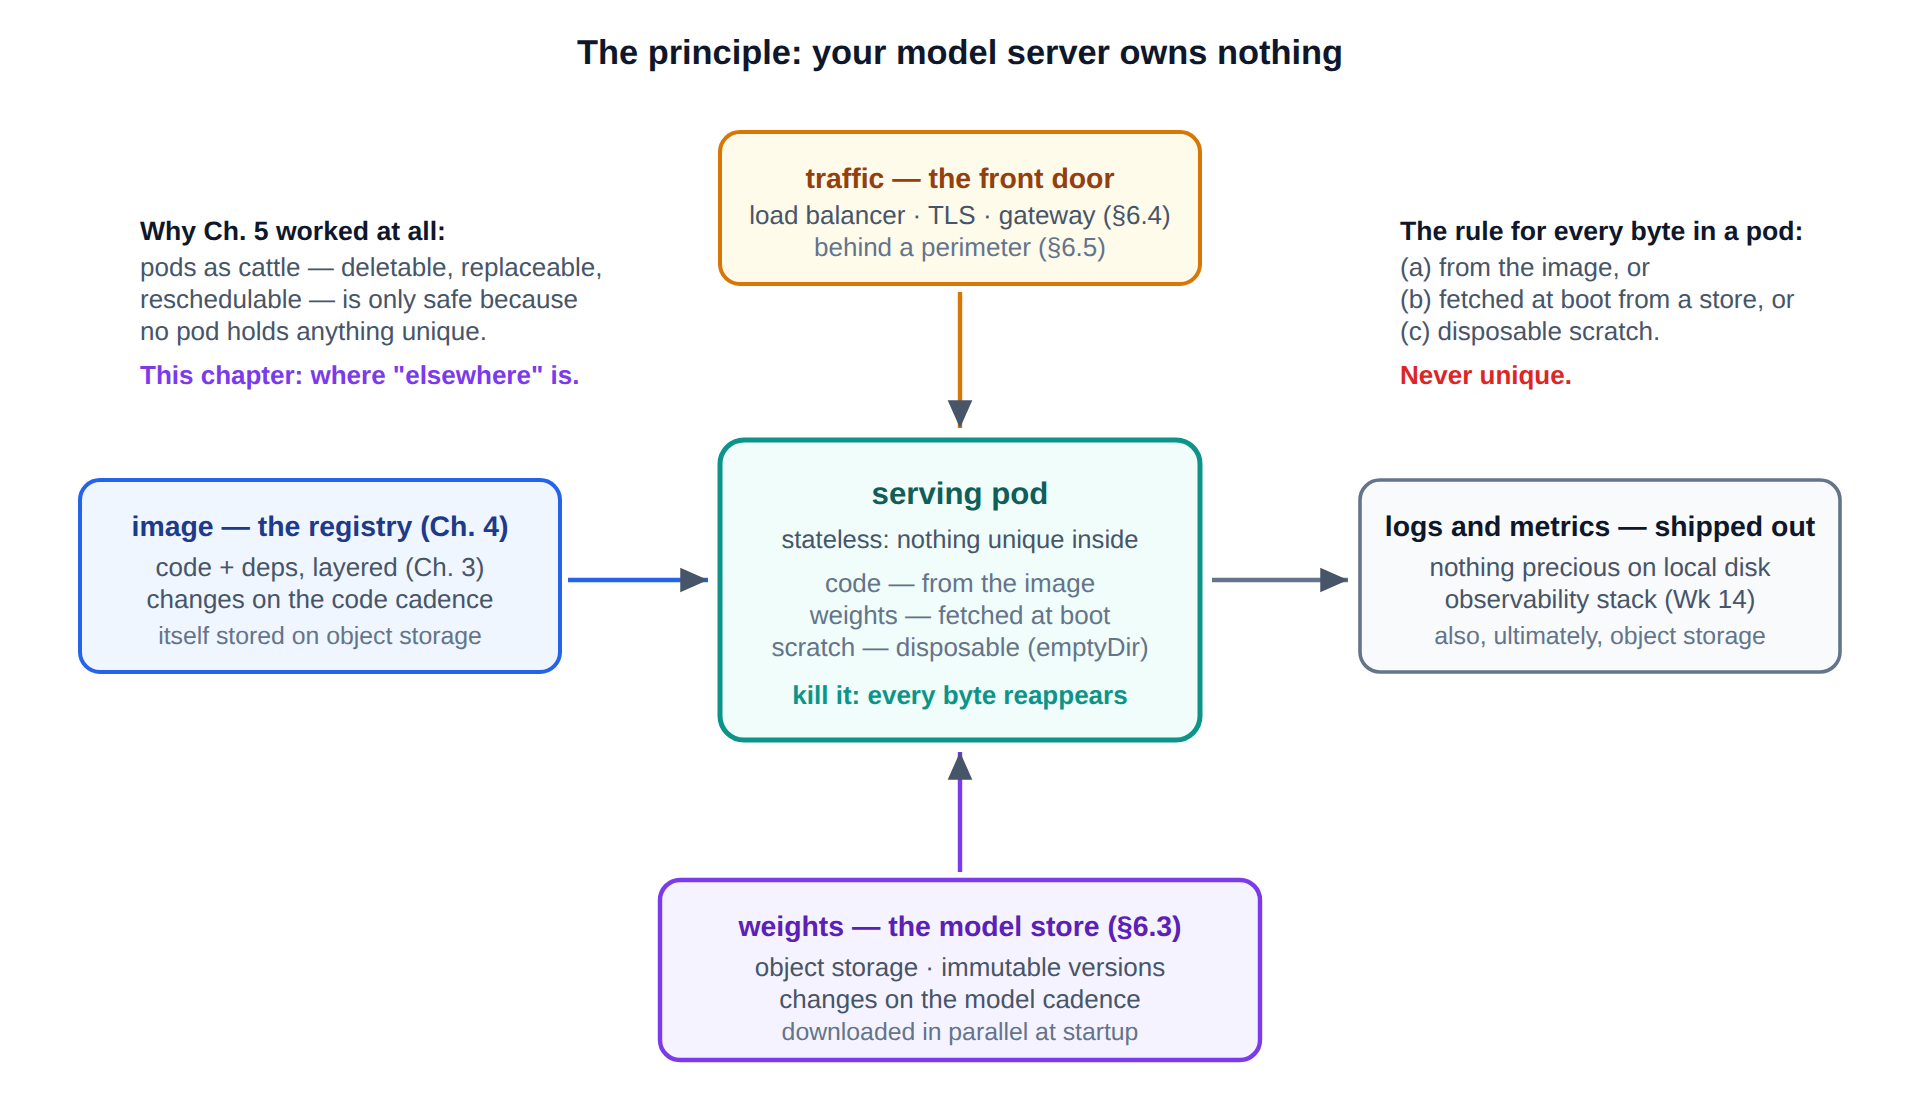
\includegraphics{figures/fig6-1_ownnothing.png}}\\[3pt]
  \figcaption{Figure 6-1  The own-nothing principle. Code arrives from the registry, weights from the model store, traffic through the front door; logs ship out. Kill the pod and every byte reappears — which is what licensed all of Chapter 5.}
\end{tbbfigure}

\subsection*{The state inventory}

"Stateless" does not mean serving systems have no state — they are drowning in it. It means the \textit{server process} holds none of it uniquely; each kind of state is pushed to a store whose contract matches its shape. It is worth being exhaustive once, because every later architecture discussion in this course is secretly a row of this table:

\begin{tbbtablewrap}
  \begin{tabular}{@{}>{\raggedright\arraybackslash}m{\dimexpr 0.2660\tbltextwidth-2\tabcolsep\relax} >{\raggedright\arraybackslash}m{\dimexpr 0.3723\tbltextwidth-2\tabcolsep\relax} >{\raggedright\arraybackslash}m{\dimexpr 0.3617\tbltextwidth-2\tabcolsep\relax}@{}}
  \arrayrulecolor{tbbnavy}\specialrule{1pt}{0pt}{0pt}
  \rowcolor{tbbtablehead}{\centering \bfseries\color{tbbnavy}State} & {\centering \bfseries\color{tbbnavy}Where it lives} & {\centering \bfseries\color{tbbnavy}Why there} \\
  \arrayrulecolor{tbbnavy}\specialrule{0.7pt}{0pt}{2pt}
  {code + dependencies} & {image, in a registry (Ch. 4)} & {versioned, content-addressed, cached per node} \\
  \arrayrulecolor{tbbtableborder}\hline
  {\textbf{model weights}} & {\textbf{the model store — object storage (§6.3)}} & {huge, immutable, versioned, read by every replica} \\
  \arrayrulecolor{tbbtableborder}\hline
  {request state} & {nowhere — in the request itself} & {stateless HTTP: any replica can answer any request} \\
  \arrayrulecolor{tbbtableborder}\hline
  {caches (tokenizer, JIT, warmup)} & {local scratch (emptyDir) — disposable} & {cheap to rebuild; never worth a pod's mortality} \\
  \arrayrulecolor{tbbtableborder}\hline
  {logs · metrics · traces} & {shipped out continuously (Wk 14)} & {the pod may die before you read them} \\
  \arrayrulecolor{tbbtableborder}\hline
  {user data · features · sessions} & {databases and feature stores} & {transactional, mutable — block-backed engines (§6.2)} \\
  \arrayrulecolor{tbbnavy}\specialrule{1pt}{2pt}{0pt}
  \end{tabular}\par
  \figcaption{Table 6-1  Where each kind of serving state belongs}
\end{tbbtablewrap}

Two rows deserve a second look. \textbf{Request state} is why Chapter 5's Service could pick "one healthy backend per connection" so casually: if any replica can answer any request, load balancing is a free choice. The moment you are tempted by session affinity ("sticky sessions"), you have usually smuggled state into the server — and bought yourself uneven load, draining problems at every rollout, and a worse failure story, which is why serving systems treat affinity as a smell rather than a feature. \textbf{Caches} are the subtle one: a warmed-up pod \textit{is} different from a cold one (Chapter 3's page cache full of weights, JIT-compiled kernels, primed allocators) — statelessness is about \textit{correctness}, not \textit{performance}. Losing a cache must never lose an answer; it may absolutely lose you latency, which is precisely why cold starts are a bill this chapter itemizes (§6.3) and Week 12 fights.

\subsection*{Why this chapter pays rent}

\begin{tbbitemize}
  \item \textbf{The weights problem is the serving problem.} A 440 MB BERT is forgiving; a 13 GB quantized LLM is not, and Week 11's models are larger still. Where weights live, how fast they arrive, and how they are versioned decides your cold-start bill (Wk 12), your deploy story (Wk 13), and a surprising share of your invoice (§6.5's NAT trap).
  \item \textbf{The front door is the product.} Chapter 5's Service has a cluster-internal name; nobody can bill a ClusterIP. TLS, routing, quotas, and metering (§6.4) are what turn a Deployment into the model API of Chapter 1's ecosystem — and the course project requires exactly this exposure, done properly.
  \item \textbf{The perimeter is not optional.} A GPU fleet is the most expensive and most attackable thing most teams run. §6.5's VPC pattern — one public door, private metal, keyless identity — is the difference between an architecture and an incident report.
  \item \textbf{This completes the infrastructure half.} After this chapter: kernel (Ch. 2–3), packaging (Ch. 4), orchestration (Ch. 5), state and edges (Ch. 6). Part 2 of the course serves models on top of this stack without looking down again — except when debugging, which is why §6.6 exists.
\end{tbbitemize}

\begin{calloutbox}{tbbpurple}{tbbpurplefill}
{\normalsize\bfseries\color{tbbpurple}Think About It}\par\vspace{3pt}
\begin{tbbitemize}
  \item Find the state hiding in most "stateless" servers: in-flight requests. Which two mechanisms from Chapters 3 and 5 exist precisely to drain that state at shutdown, and what breaks if you skip them?
  \item A teammate proposes sticky sessions so each user's requests hit the same replica ("the KV cache will be warm"). Enumerate what this costs at rollout time, at autoscale-down, and at node failure — then note where this exact tension returns for real in Week 11 (LLM sessions).
  \item Suppose weights were baked into the image instead (Ch. 3 §3.4's anti-pattern). Walk Table 6-1's image row and list which properties silently break: what does "versioned" now mean, what does a code hotfix cost, what does the registry bill look like at 13 GB × weekly deploys?
\end{tbbitemize}
\end{calloutbox}

\section{Two Contracts: Block and Object}

Cloud storage comes in three families, and the productive way to compare them is not by feature list but by \textbf{contract} — what the service promises, and what it charges for the promise. Get the contracts straight once and every storage decision in this course reduces to pattern-matching: what is the access pattern, who shares it, how durable must it be, and which contract sells exactly that (Figure 6-2).

\subsection*{Block: a disk you attach}

\textbf{Block storage} (AWS EBS, GCP Persistent Disk) sells the oldest promise in computing: \textit{a disk}. You are given a raw device of a size you chose; the OS cannot tell it from local hardware — it is, in fact, Chapter 2's virtio story again, a paravirtual disk whose blocks live on replicated storage servers across the network. You put a filesystem on it and get full POSIX semantics: random reads and writes, in-place updates, byte-level seeks, sub-millisecond-to-millisecond latency. This is the contract databases require — a B-tree wants to rewrite page 4,381 in place, ten thousand times a second — and the contract is priced accordingly: you \textbf{provision} capacity and performance (size in GB, IOPS, throughput) and pay for what you reserved whether you use it or not (gp3-class: \textasciitilde{}\$0.08/GB-month, representative). Two fine-print clauses matter operationally: a block volume attaches to \textbf{one instance at a time} (it is a disk, not a share), and it lives in \textbf{one availability zone} — durability beyond that is your job, via snapshots (which land, pleasingly, on object storage).

\begin{terminalbox}
\begin{Verbatim}[breaklines=true,breakanywhere=true,fontsize=\small,formatcom=\color{tbbtermfg},codes=\tbbcodeactive]
$ lsblk
NAME     SIZE  TYPE  MOUNTPOINT
nvme0n1  100G  disk  /              # boot volume (also block!)
nvme1n1  200G  disk                 # the EBS volume we attached
$ sudo mkfs.ext4 /dev/nvme1n1 && sudo mount /dev/nvme1n1 /scratch
$ dd if=/dev/zero of=/scratch/t bs=4k count=1 oflag=dsync
4096 bytes copied, 0.00089 s      # ~0.9 ms: a disk-shaped latency
# the OS cannot tell this from local hardware. that is the product.
\end{Verbatim}
\end{terminalbox}
\figcaption{Transcript 6-2  The block contract, felt: attach, format, mount — and sub-millisecond writes. Chapter 2's virtio machinery is under every line.}

\subsection*{Object: an API you call}

\textbf{Object storage} (S3, GCS) sells a completely different promise: \textit{durable blobs behind an HTTP API}. There is no device, no filesystem, no seek. You \code{PUT} an object (up to 5 TB) under a key like \code{bert-classifier/\allowbreak v7/\allowbreak model.safetensors}, and you \code{GET} it back — whole, or any byte range of it. What you cannot do is edit in place: there is no "overwrite bytes 100–200 of an object"; you replace the whole object or you do not touch it. In exchange for giving up disk semantics, you get properties no disk can offer. \textbf{Durability}: eleven nines (99.999999999\%), achieved by erasure-coding every object across devices and availability zones — losing an object is headline material, and nobody snapshots S3. \textbf{Scale and sharing}: capacity is unlimited and \textit{every} reader in the region can fetch simultaneously; a thousand pods pulling the same weights is a Tuesday. \textbf{Price}: pay for what is actually stored (\textasciitilde{}\$0.023/GB-month standard class), per request (\textasciitilde{}\$0.0004 per 1,000 GETs), and — the clause everyone forgets — \textbf{per byte leaving} (egress to the internet \textasciitilde{}\$0.09/GB; §6.5 adds the NAT wrinkle). The latency fine print: \textbf{time-to-first-byte is tens of milliseconds} — a hundred times a disk — but each stream then delivers 50–100 MB/s, and streams multiply. Ask for many ranges of many objects in parallel and object storage will happily saturate a 10 Gbps NIC. Slow to start, unbounded in aggregate: remember that shape; §6.3 is built on it.

\begin{terminalbox}
\begin{Verbatim}[breaklines=true,breakanywhere=true,fontsize=\small,formatcom=\color{tbbtermfg},codes=\tbbcodeactive]
$ aws s3 cp model.safetensors s3://ml-models/bert-classifier/v7/
upload: ./model.safetensors to s3://ml-models/.../model.safetensors
$ curl -sI "$(aws s3 presign s3://ml-models/.../model.safetensors)" \
    -H "Range: bytes=0-1048575" | grep -E "HTTP|Content-Range"
HTTP/1.1 206 Partial Content
Content-Range: bytes 0-1048575/461301120
# a ranged GET: any slice of any object, over plain HTTPS.
# no mount, no filesystem, no single owner - and 206 is the
# status code your parallel loader (sec. 6.3) lives on.
\end{Verbatim}
\end{terminalbox}
\figcaption{Transcript 6-3  The object contract, felt: upload is an HTTP PUT; a presigned URL plus a Range header fetches any megabyte of a 440 MB object. Parallelism is just more of these.}

Two more clauses complete the contract. \textbf{Consistency}: S3 has been strongly consistent since 2020 — a \code{GET} after a \code{PUT} returns the new object, full stop — which retired a decade of folklore workarounds; the discipline §6.3 builds (immutable versions) is therefore about \textit{operational} sanity, not consistency bugs. \textbf{Tiers}: the same API fronts multiple \textbf{storage classes} (standard → infrequent-access → archive) with falling storage prices and rising retrieval costs; \textbf{lifecycle rules} move objects between them by age. For a model store this matters at the fleet level: last year's 400 model versions do not deserve standard-class pricing, and a one-line lifecycle rule ("non-current versions → infrequent access after 30 days") is the difference between a tidy bill and a growing one.

\subsection*{File, PersistentVolumes, and the honest table}

The third family, \textbf{file storage} (NFS as a service: EFS, Filestore), is the compromise contract: POSIX semantics \textit{and} many concurrent readers/writers, purchased at roughly four times block's price per gigabyte and with network-filesystem latency. It earns its keep where many pods must share \textit{mutable} files — a shared cache that several trainers append to — and it is routinely mis-bought where an object store plus local caches would be cheaper and faster. In Kubernetes, block and file surface as \textbf{PersistentVolumes}: a PVC with \code{ReadWriteOnce} (RWO) access is block — one node at a time, exactly the disk contract — while \code{ReadWriteMany} (RWX) is file. Object storage, tellingly, does not appear in this list at all: it is not a volume you mount but an API you call, which is precisely why it can be shared by a thousand readers without a filesystem in the way. (FUSE adapters that mount buckets as filesystems exist — s3fs, mountpoint — and are handy for exploration; treat them as convenience shims, not as a way to make object storage keep disk promises it never made.)

\begin{tbbtablewrap}
  \begin{tabular}{@{}>{\raggedright\arraybackslash}m{\dimexpr 0.2181\tbltextwidth-2\tabcolsep\relax} >{\raggedright\arraybackslash}m{\dimexpr 0.2660\tbltextwidth-2\tabcolsep\relax} >{\raggedright\arraybackslash}m{\dimexpr 0.2766\tbltextwidth-2\tabcolsep\relax} >{\raggedright\arraybackslash}m{\dimexpr 0.2394\tbltextwidth-2\tabcolsep\relax}@{}}
  \arrayrulecolor{tbbnavy}\specialrule{1pt}{0pt}{0pt}
  \rowcolor{tbbtablehead}{\centering \bfseries\color{tbbnavy}} & {\centering \bfseries\color{tbbnavy}Block (EBS)} & {\centering \bfseries\color{tbbnavy}Object (S3)} & {\centering \bfseries\color{tbbnavy}File (EFS)} \\
  \arrayrulecolor{tbbnavy}\specialrule{0.7pt}{0pt}{2pt}
  {\textbf{you get}} & {a raw disk} & {an HTTP API over blobs} & {a shared POSIX tree} \\
  \arrayrulecolor{tbbtableborder}\hline
  {\textbf{semantics}} & {random R/W in place} & {PUT/GET whole or ranges; no edit} & {POSIX, concurrent} \\
  \arrayrulecolor{tbbtableborder}\hline
  {\textbf{latency}} & {sub-ms – ms} & {\textasciitilde{}tens of ms first byte} & {ms (network hop)} \\
  \arrayrulecolor{tbbtableborder}\hline
  {\textbf{throughput}} & {provisioned, per volume} & {\textbf{parallel: to NIC saturation}} & {provisioned/bursting} \\
  \arrayrulecolor{tbbtableborder}\hline
  {\textbf{sharing}} & {one instance (RWO)} & {unlimited readers} & {many R/W (RWX)} \\
  \arrayrulecolor{tbbtableborder}\hline
  {\textbf{durability}} & {one AZ + your snapshots} & {\textbf{eleven nines, cross-AZ}} & {multi-AZ, managed} \\
  \arrayrulecolor{tbbtableborder}\hline
  {\textbf{price shape}} & {\textasciitilde{}\$0.08/GB-mo provisioned} & {\textasciitilde{}\$0.023/GB-mo + requests + egress} & {\textasciitilde{}\$0.30/GB-mo used} \\
  \arrayrulecolor{tbbtableborder}\hline
  {\textbf{serving home}} & {databases · node scratch} & {\textbf{weights · datasets · images · logs}} & {shared mutable caches} \\
  \arrayrulecolor{tbbnavy}\specialrule{1pt}{2pt}{0pt}
  \end{tabular}\par
  \figcaption{Table 6-2  The three contracts, side by side (representative prices)}
\end{tbbtablewrap}

\begin{calloutbox}{tbbblue}{tbbbluefill}
{\normalsize\bfseries\color{tbbblue}Worked example — one 13 GB model, four ways}\par\vspace{3pt}
A 13 GB model must be available to 20 replicas across 5 nodes. Compare monthly storage cost and behavior (representative prices):

\begin{tbbitemize}
  \item \textbf{Object store (the pattern):} one copy: 13 GB × \$0.023 ≈ \textbf{\$0.30/mo}, plus pennies of GET requests per deploy. Every node caches locally on first pull (block scratch it already has). Versioning: new prefix, free-ish.
  \item \textbf{Per-node block volumes:} 5 × 13 GB × \$0.08 ≈ \textbf{\$5.20/mo}, plus the orchestration you now own: getting new versions onto 5 disks, atomically, with rollback. You have reinvented a worse model store.
  \item \textbf{File share:} 13 GB × \$0.30 ≈ \textbf{\$3.90/mo}, shared mount, easy — until 20 replicas cold-start together and contend on one share's throughput; and you still need versioning discipline.
  \item \textbf{Baked into the image (Ch. 3's anti-pattern):} storage is cheap (registries sit on object storage anyway) but every code deploy re-ships 13 GB × 5 nodes through the registry path, and model version is now welded to image version — the real cost is workflow, not gigabytes.
\end{tbbitemize}

The pattern that wins is a composite: \textbf{object store as the source of truth, block as the per-node cache} — store once, cache locally, version by prefix. That composite has a name; it is the next section.
\end{calloutbox}

\vspace{3.0pt}

\begin{tbbfigure}
  \adjustbox{max width=0.94\linewidth,max totalheight=0.46\textheight}{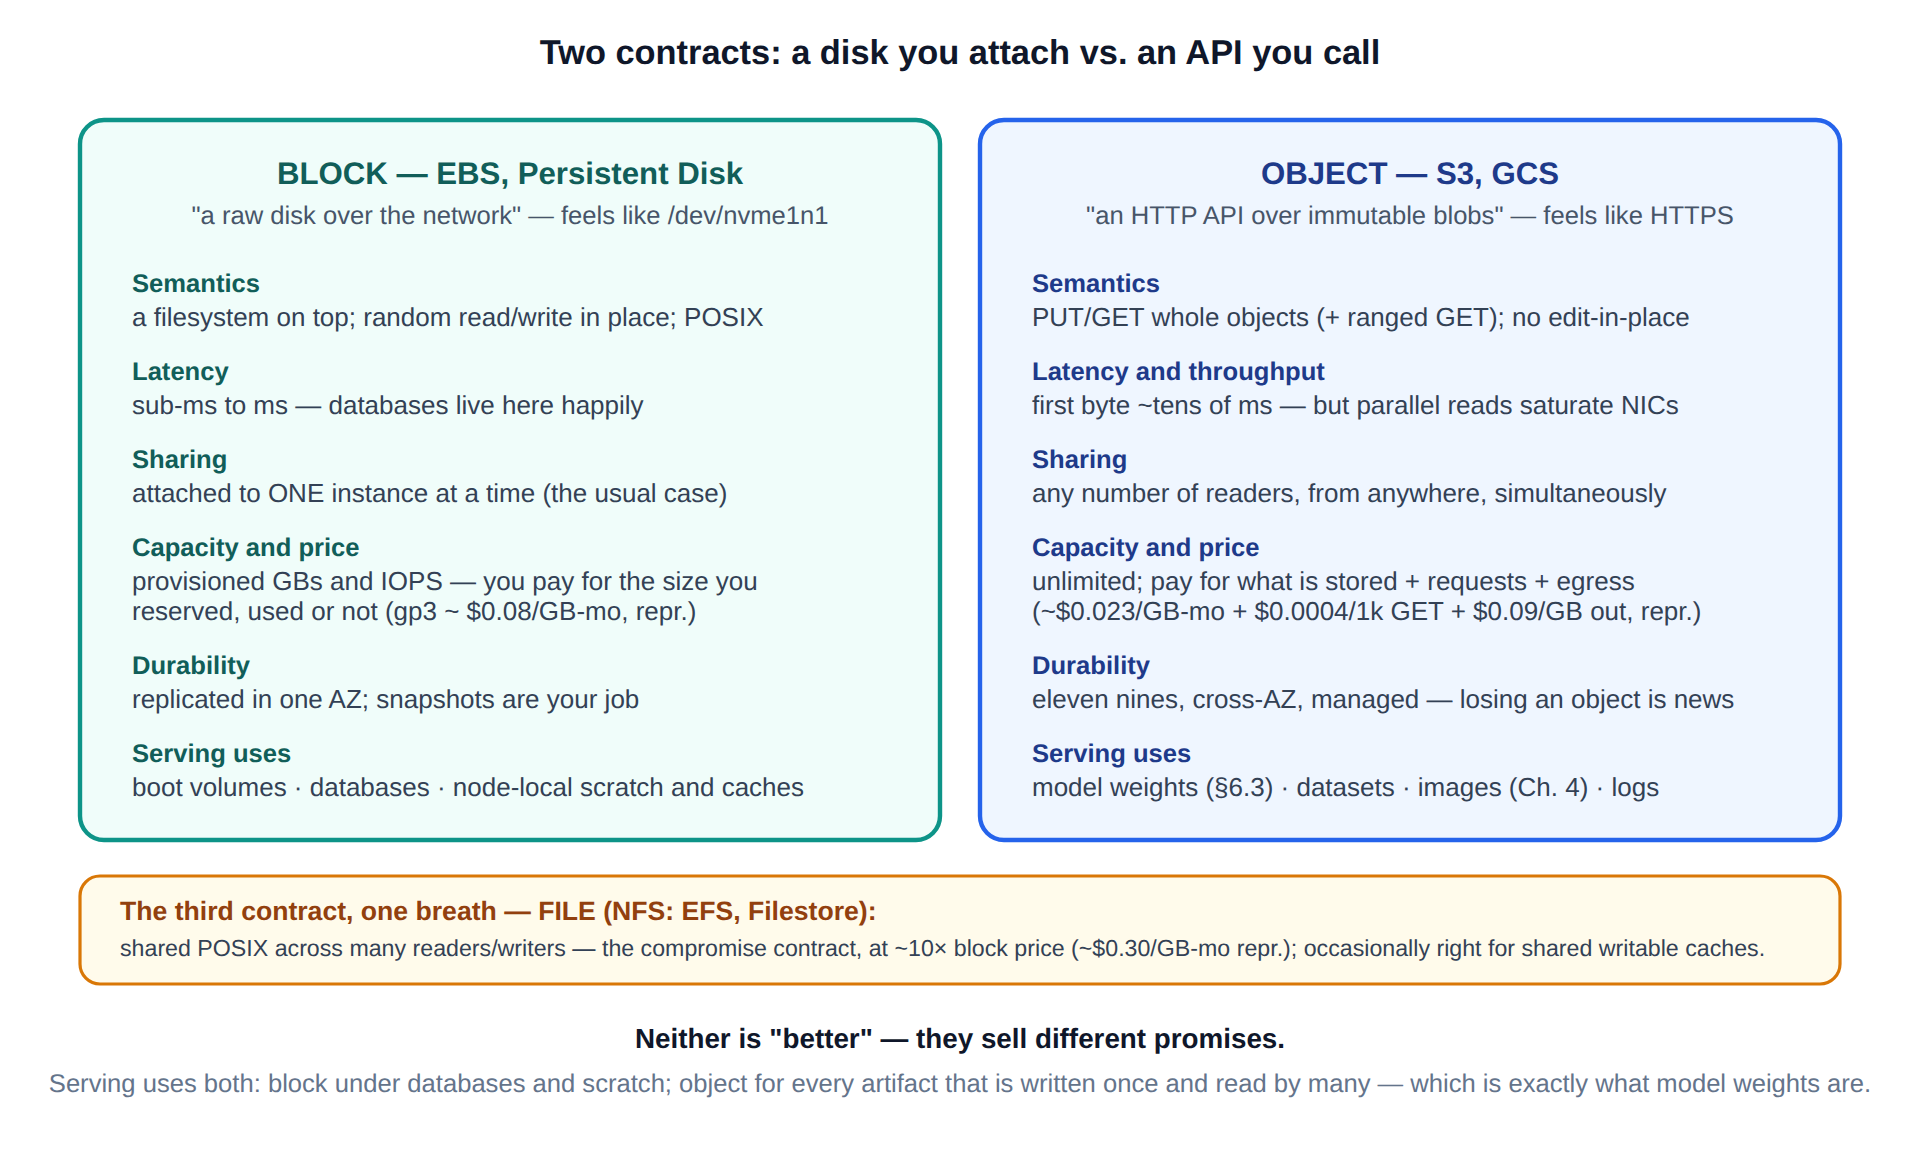
\includegraphics{figures/fig6-2_contracts.png}}\\[3pt]
  \figcaption{Figure 6-2  Two contracts: block sells a disk (POSIX, microseconds, one owner); object sells durable blobs behind HTTP (ranged reads, unlimited readers, parallel throughput). File is the pricey compromise.}
\end{tbbfigure}

\begin{calloutbox}{tbbpurple}{tbbpurplefill}
{\normalsize\bfseries\color{tbbpurple}Think About It}\par\vspace{3pt}
\begin{tbbitemize}
  \item A PostgreSQL database on object storage is a terrible idea; analytics engines happily query Parquet files on S3 all day. What changed between the two workloads? Name the two contract clauses that decide it.
  \item S3 promises eleven nines of durability but a much weaker availability SLA (\textasciitilde{}99.9\%). What is the difference, and what does the gap force your loader (§6.3) to do?
  \item Your team wants one RWX file share holding "the current model," updated in place at each release. It works in the demo. List three ways it hurts you within a quarter (think: mid-download updates, rollback, cold-start contention).
\end{tbbitemize}
\end{calloutbox}

\section{The Model Store}

Chapter 3 §3.4 ended with a promissory note: \textit{"model weights usually do not belong in image layers — they live properly in a model store, loaded at startup."} This section pays it. The argument is a perfect fit between a workload and a contract: weights are \textbf{huge} (hundreds of MB to hundreds of GB), \textbf{immutable} (a trained artifact never changes — a new train is a new artifact), \textbf{versioned} (you will keep many and switch between them), \textbf{written once and read by every replica}, and consumed as \textbf{large sequential reads} that parallelize beautifully. Reread §6.2's object contract: that is the same list. Weights are the most object-shaped bytes in your entire system (Figure 6-3).

\begin{tbbfigure}
  \adjustbox{max width=0.94\linewidth,max totalheight=0.46\textheight}{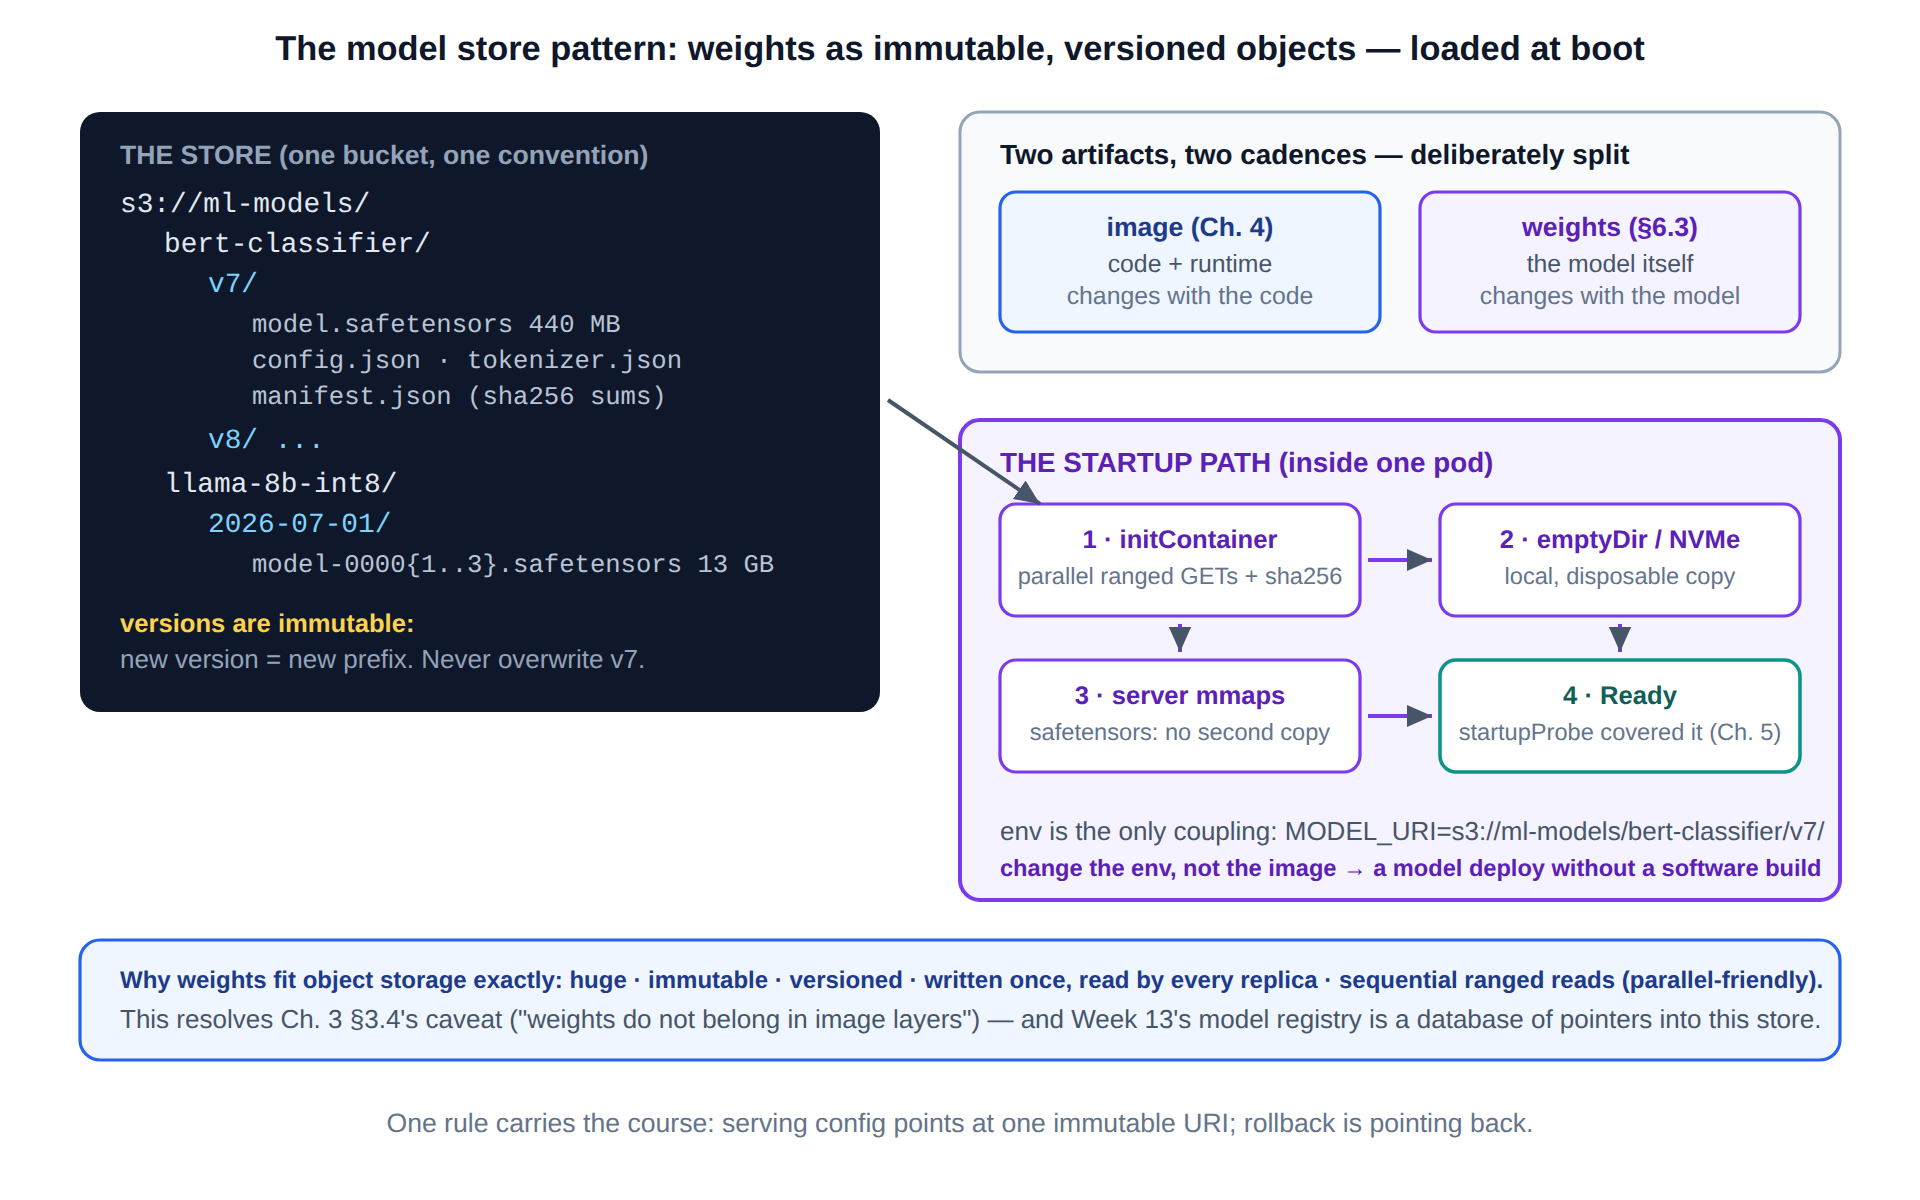
\includegraphics{figures/fig6-3_modelstore.png}}\\[3pt]
  \figcaption{Figure 6-3  The model store: one bucket, one naming convention, immutable versions — and the startup path that turns a URI into a served model. The env var is the only coupling between image and weights.}
\end{tbbfigure}

\subsection*{Layout: one convention, enforced with immutability}

\begin{terminalbox}
\begin{Verbatim}[breaklines=true,breakanywhere=true,fontsize=\small,formatcom=\color{tbbtermfg},codes=\tbbcodeactive]
$ aws s3 ls s3://ml-models/ --recursive --human-readable | head -12
bert-classifier/v7/model.safetensors        440.0 MiB
bert-classifier/v7/config.json                1.2 KiB
bert-classifier/v7/tokenizer.json           695.4 KiB
bert-classifier/v7/manifest.json              0.6 KiB
bert-classifier/v8/model.safetensors        440.1 MiB
bert-classifier/v8/...
llama-8b-int8/2026-07-01/model-00001.safetensors  4.9 GiB
llama-8b-int8/2026-07-01/model-00002.safetensors  4.9 GiB
llama-8b-int8/2026-07-01/model-00003.safetensors  3.4 GiB
llama-8b-int8/2026-07-01/manifest.json            0.7 KiB
$ cat manifest.json   # (from v7)
{ "model": "bert-classifier", "version": "v7",
  "files": { "model.safetensors":
    "sha256:9f2c4a01..." },
  "trained": "2026-06-14", "framework": "torch-2.6" }
\end{Verbatim}
\end{terminalbox}
\figcaption{Transcript 6-4  The store's whole schema: model/version/files, plus a manifest whose sha256 sums make every download verifiable. Rhymes deliberately with Chapter 4's content-addressed image layers.}

The layout is almost embarrassingly simple — \code{<model>/\allowbreak <version>/\allowbreak <files>} — and the entire pattern rests on one discipline: \textbf{versions are immutable.} A new training run, a new quantization, even a fixed tokenizer file: new prefix. Never, under any deadline, overwrite \code{v7/\allowbreak } in place. The reasons compound. A rolling update (Chapter 5) has old and new pods running side by side for minutes — if \code{v7} can change underneath them, replicas \textit{of the same declared version} disagree. Node caches (below) key on the URI — mutate the contents and every cache is silently poisoned. Rollback (Chapter 5's \code{rollout undo}, Week 13's automation) only means anything if the thing you roll back to still exists, unmodified. And the \code{manifest.json}'s checksums give every consumer a self-verifying download — the same integrity idea as Chapter 4's image digests, applied one artifact up the stack. Immutability turns "which model is running?" from an investigation into a string comparison: the URI \textit{is} the answer.

\subsection*{Loading fast: the parallel loader}

Now the performance half. Recall the object contract's shape — slow first byte, unbounded aggregate — and look at what a naive loader does: one \code{GET}, one stream, \textasciitilde{}80 MB/s if you are lucky. For 13 GB that is \textbf{162 seconds} of a GPU node doing nothing billable. The fix is to \textit{use the contract}: split each object into ranges, fetch 8–16 ranges concurrently (Transcript 6-3's \code{206 Partial Content}, multiplied), and write them into place. Aggregate throughput climbs until you hit the \textbf{NIC} (10 Gbps ≈ 1.25 GB/s ceiling) or local disk — S3 itself will not be your bottleneck at this scale, and it explicitly supports massive request parallelism per prefix. Purpose-built tools (\code{s5cmd}, the AWS CLI's configurable concurrency, \code{hf\_transfer}) all implement exactly this; the lab has you write a minimal one so the mechanism is yours:

\begin{terminalbox}
\begin{Verbatim}[breaklines=true,breakanywhere=true,fontsize=\small,formatcom=\color{tbbtermfg},codes=\tbbcodeactive]
# the experiment the lab reproduces (13 GB, same node, same bucket):
$ time python loader.py --streams 1 $MODEL_URI /models
real  2m42.1s                       # ~80 MB/s: one stream
$ time python loader.py --streams 16 $MODEL_URI /models
real  0m16.8s                       # ~790 MB/s: sixteen ranged streams
# 9.6x from the same bucket, same NIC - the contract, exploited.
$ sha256sum -c <(python manifest_sums.py /models/manifest.json)
model-00001.safetensors: OK
model-00002.safetensors: OK
model-00003.safetensors: OK        # verify before you serve. always.
\end{Verbatim}
\end{terminalbox}
\figcaption{Transcript 6-5  The parallel loader: 162 s → 17 s by turning one GET into sixteen ranged GETs — then checksum verification against the manifest before a single request is served.}

After download comes \textbf{load}, and one format choice makes it nearly free: \textbf{safetensors}. The format is a JSON header (tensor names, dtypes, shapes, offsets) followed by raw tensor bytes — designed so a loader can \code{mmap} the file and use tensors \textit{in place}, zero-copy, rather than deserializing (and unlike pickle-based checkpoints, opening one cannot execute code — the security half of Week 7's format discussion). The Chapter 3 payoff is satisfying: an mmapped weight file is \textbf{file-backed page cache} — the kernel pages tensors in on first touch and can reclaim them under pressure, which is why a healthy model server's \code{memory.current} hugs its limit while \code{anon} stays modest (§3.3's dashboard lesson, now with a cause you engineered). For GPU serving the sequence continues — host pages then copied to VRAM — and Week 10's optimization chapter picks up from there.

\subsection*{Wiring it into the pod: initContainer, emptyDir, and a probe that knows}

\begin{terminalbox}
\begin{Verbatim}[breaklines=true,breakanywhere=true,fontsize=\small,formatcom=\color{tbbtermfg},codes=\tbbcodeactive]
    spec:
      volumes:
      - name: models
        emptyDir: {}              # node-local scratch; dies with pod
      initContainers:
      - name: fetch-model
        image: registry.example.com/team/model-loader:v3
        args: ["$(MODEL_URI)", "/models", "--streams", "16"]
        env:
        - { name: MODEL_URI,
            value: "s3://ml-models/bert-classifier/v7/" }
        volumeMounts: [ { name: models, mountPath: /models } ]
      containers:
      - name: server
        image: registry.example.com/team/model-server:v12
        env:
        - { name: MODEL_DIR, value: "/models" }
        volumeMounts: [ { name: models, mountPath: /models } ]
        startupProbe:             # budget = download + load + margin
          httpGet: { path: /healthz, port: 8000 }
          periodSeconds: 5
          failureThreshold: 24    # 24 x 5s = 2 min for the 440 MB case
\end{Verbatim}
\end{terminalbox}
\figcaption{Transcript 6-6  The wiring: an initContainer downloads into an emptyDir before the server starts; the startupProbe budget (Ch. 5) is now a number you compute from Transcript 6-5's measurements.}

Each piece is doing one deliberate job. The \textbf{initContainer} runs to completion \textit{before} the server container starts — so the server's image stays free of loader dependencies, download failures surface as a distinct \code{Init:Error} state (cleanly separable in Chapter 5's field guide), and the loader can be upgraded independently. The \textbf{emptyDir} is honest scratch: it lives exactly as long as the pod, on node disk (or \code{medium: Memory} when you want tmpfs), and its deletion with the pod is not a bug but the own-nothing principle enforced by the platform. The \textbf{startupProbe} budget stops being folklore and becomes arithmetic: measured download (17 s) + load (10 s) + margin → threshold. And the \textbf{env var is the only coupling}: the server reads \code{/\allowbreak models}, the initContainer fills it from \code{MODEL\_URI}, and \textit{neither image mentions a model version}. Which sets up the best transcript in the chapter:

\begin{terminalbox}
\begin{Verbatim}[breaklines=true,breakanywhere=true,fontsize=\small,formatcom=\color{tbbtermfg},codes=\tbbcodeactive]
$ kubectl set env deploy/model-server MODEL_URI=s3://ml-models/bert-classifier/v8/
deployment.apps/model-server env updated
$ kubectl rollout status deploy/model-server && kubectl get pods \
    -o custom-columns=NAME:.metadata.name,IMAGE:.spec.containers[0].image
deployment "model-server" successfully rolled out
NAME                            IMAGE
model-server-59d8c7f9b6-2xk4p   registry.example.com/team/model-server:v12
model-server-59d8c7f9b6-m7qvw   registry.example.com/team/model-server:v12
model-server-59d8c7f9b6-tt8zn   registry.example.com/team/model-server:v12
# same image. new model. a rolling, health-gated, rollback-able
# model deploy (Ch. 5 machinery) - and no software was built.
\end{Verbatim}
\end{terminalbox}
\figcaption{Transcript 6-7  The payoff: a model deploy is now an env change — surged, readiness-gated, and revertible like any Chapter 5 rollout, with the IMAGE column untouched. Week 13 automates exactly this line.}

Pause on what just happened, because it is the architectural point of the whole chapter. By splitting the two cadences — code in images, weights in the store — a \textbf{model release stopped being a software release.} No Dockerfile, no CI build, no registry push; the "deploy" is one field, and every safety mechanism Chapter 5 built (surge, readiness pacing, stalls on failure, one-command rollback) applies unchanged because it \textit{is} a Chapter 5 rollout. Week 13's model registry formalizes the bookkeeping (which URI is "staging", which is "prod", who promoted it and when), but the registry is metadata; the mechanism is this transcript.

\subsection*{The cold-start bill — and the caching ladder}

\begin{tbbfigure}
  \adjustbox{max width=0.94\linewidth,max totalheight=0.46\textheight}{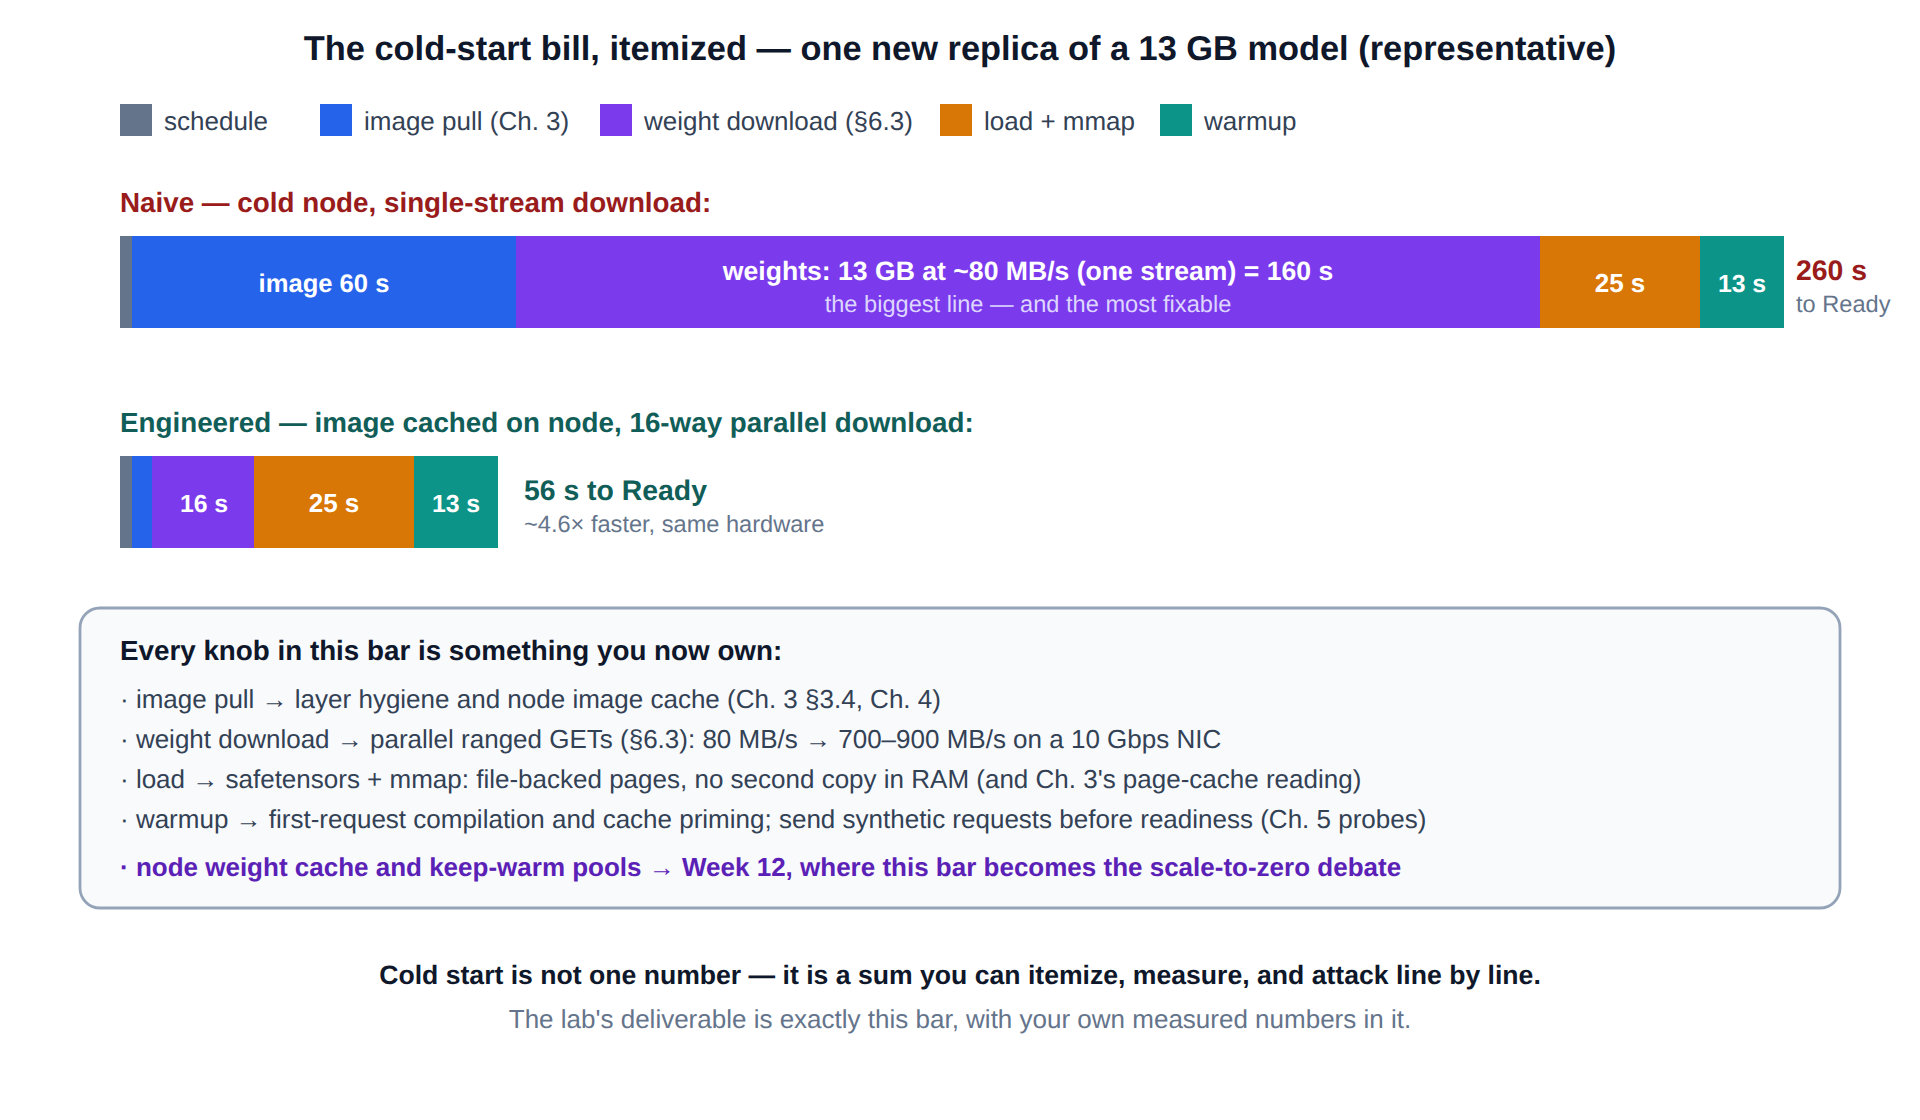
\includegraphics{figures/fig6-4_coldstart.png}}\\[3pt]
  \figcaption{Figure 6-4  The cold-start bill for one new replica, itemized. The naive bar is dominated by a single-stream download; the engineered bar gets the same replica Ready 4.6× sooner. Week 12 fights over this bar.}
\end{tbbfigure}

\begin{calloutbox}{tbbamber}{tbbamberfill}
{\normalsize\bfseries\color{tbbamberdark}Worked example — itemizing one replica's cold start (13 GB model)}\par\vspace{3pt}
Add the lines, twice (representative numbers; the lab measures yours):

\begin{tbbitemize}
  \item \textbf{Naive:} schedule \textasciitilde{}2 s + image pull 60 s (6 GB, cold node — Ch. 3's math) + weights 162 s (single stream) + load 25 s + warmup 13 s ≈ \textbf{260 s to Ready.}
  \item \textbf{Engineered:} schedule \textasciitilde{}2 s + image \textasciitilde{}0 s (cached on node) + weights 17 s (16 streams) + load 25 s + warmup 13 s ≈ \textbf{56 s to Ready.}
\end{tbbitemize}

Same hardware, 4.6× — and every line has an owner you now know: image → layer hygiene and node caches (Ch. 3–4); download → this section's loader; load → safetensors + mmap; warmup → synthetic requests before readiness (Ch. 5's probes, §6.4's health path). The remaining moves — per-node weight caches shared across pods, pre-warmed pools, and the scale-to-zero argument this bar decides — are Week 12's chapter, and it will assume this arithmetic cold.
\end{calloutbox}

\vspace{3.0pt}

The caching ladder is worth one paragraph now. The emptyDir pattern re-downloads per \textbf{pod}; a \code{hostPath}/PVC cache keyed by URI re-downloads per \textbf{node} (immutability makes this safe — a version can never be stale, only absent); a pre-pulling DaemonSet warms nodes \textbf{before} pods arrive; and baking weights into the image remains the legitimate \textit{edge case} (air-gapped deployments, demo appliances) that Chapter 3 already filed under "a decision, not a default." Each rung trades storage duplication for startup latency — the recurring trade of this course, purchasable by the gigabyte.

One last inhabitant of the store: \textbf{datasets}. Training data, evaluation sets, and the golden-request fixtures your team will use for regression testing (Week 13's CI gate) live under the same bucket discipline — versioned prefixes, manifests, immutability — usually in Parquet or JSONL. They share none of the serving path's latency drama, which is exactly why they need no new machinery: the store does not care, and that is the point.

\begin{calloutbox}{tbbpurple}{tbbpurplefill}
{\normalsize\bfseries\color{tbbpurple}Think About It}\par\vspace{3pt}
\begin{tbbitemize}
  \item Your on-call inherits an incident: after a "quick fix" someone re-uploaded v7's tokenizer.json in place. Half the replicas were restarted since. Describe the symptom zoo (same URI, two behaviors), why caches make it worse, and the one-line policy that would have prevented it.
  \item The manifest's sha256 protects against something TLS does not, and TLS protects against something the manifest does not. Name both threats precisely.
  \item A 100-replica scale-out event (Wk 12) makes every new pod pull 13 GB at once. Where does the bottleneck actually land — S3, the per-node NIC, or the node cache — under (a) emptyDir-per-pod, (b) node cache, (c) pre-warmed nodes? Show the arithmetic for one 10 Gbps node running 4 pods.
\end{tbbitemize}
\end{calloutbox}

\section{The Front Door: Load Balancers, Ingress, Gateways}

Chapter 5's exposure ladder ended at \code{type: LoadBalancer} — a raw cloud pipe to your Service, which is genuinely all a demo needs. Production asks a longer list of the front door: \textbf{TLS} (nobody posts inference inputs over plaintext), \textbf{routing} (one door, many services: \code{/\allowbreak predict} here, \code{/\allowbreak embed} there, \code{staging.api.example.com} elsewhere), \textbf{authentication and quotas} (Chapter 1's model-API economy runs on keys and meters), \textbf{timeouts and retries chosen on purpose} (inference has a tail like nothing else behind an LB), and \textbf{observability at the edge} (the status codes §6.6 reads). This section builds the door in three layers — load balancer, Ingress, gateway — and then spends deliberate time on the settings that break model serving specifically (Figure 6-5).

\begin{tbbfigure}
  \adjustbox{max width=0.94\linewidth,max totalheight=0.46\textheight}{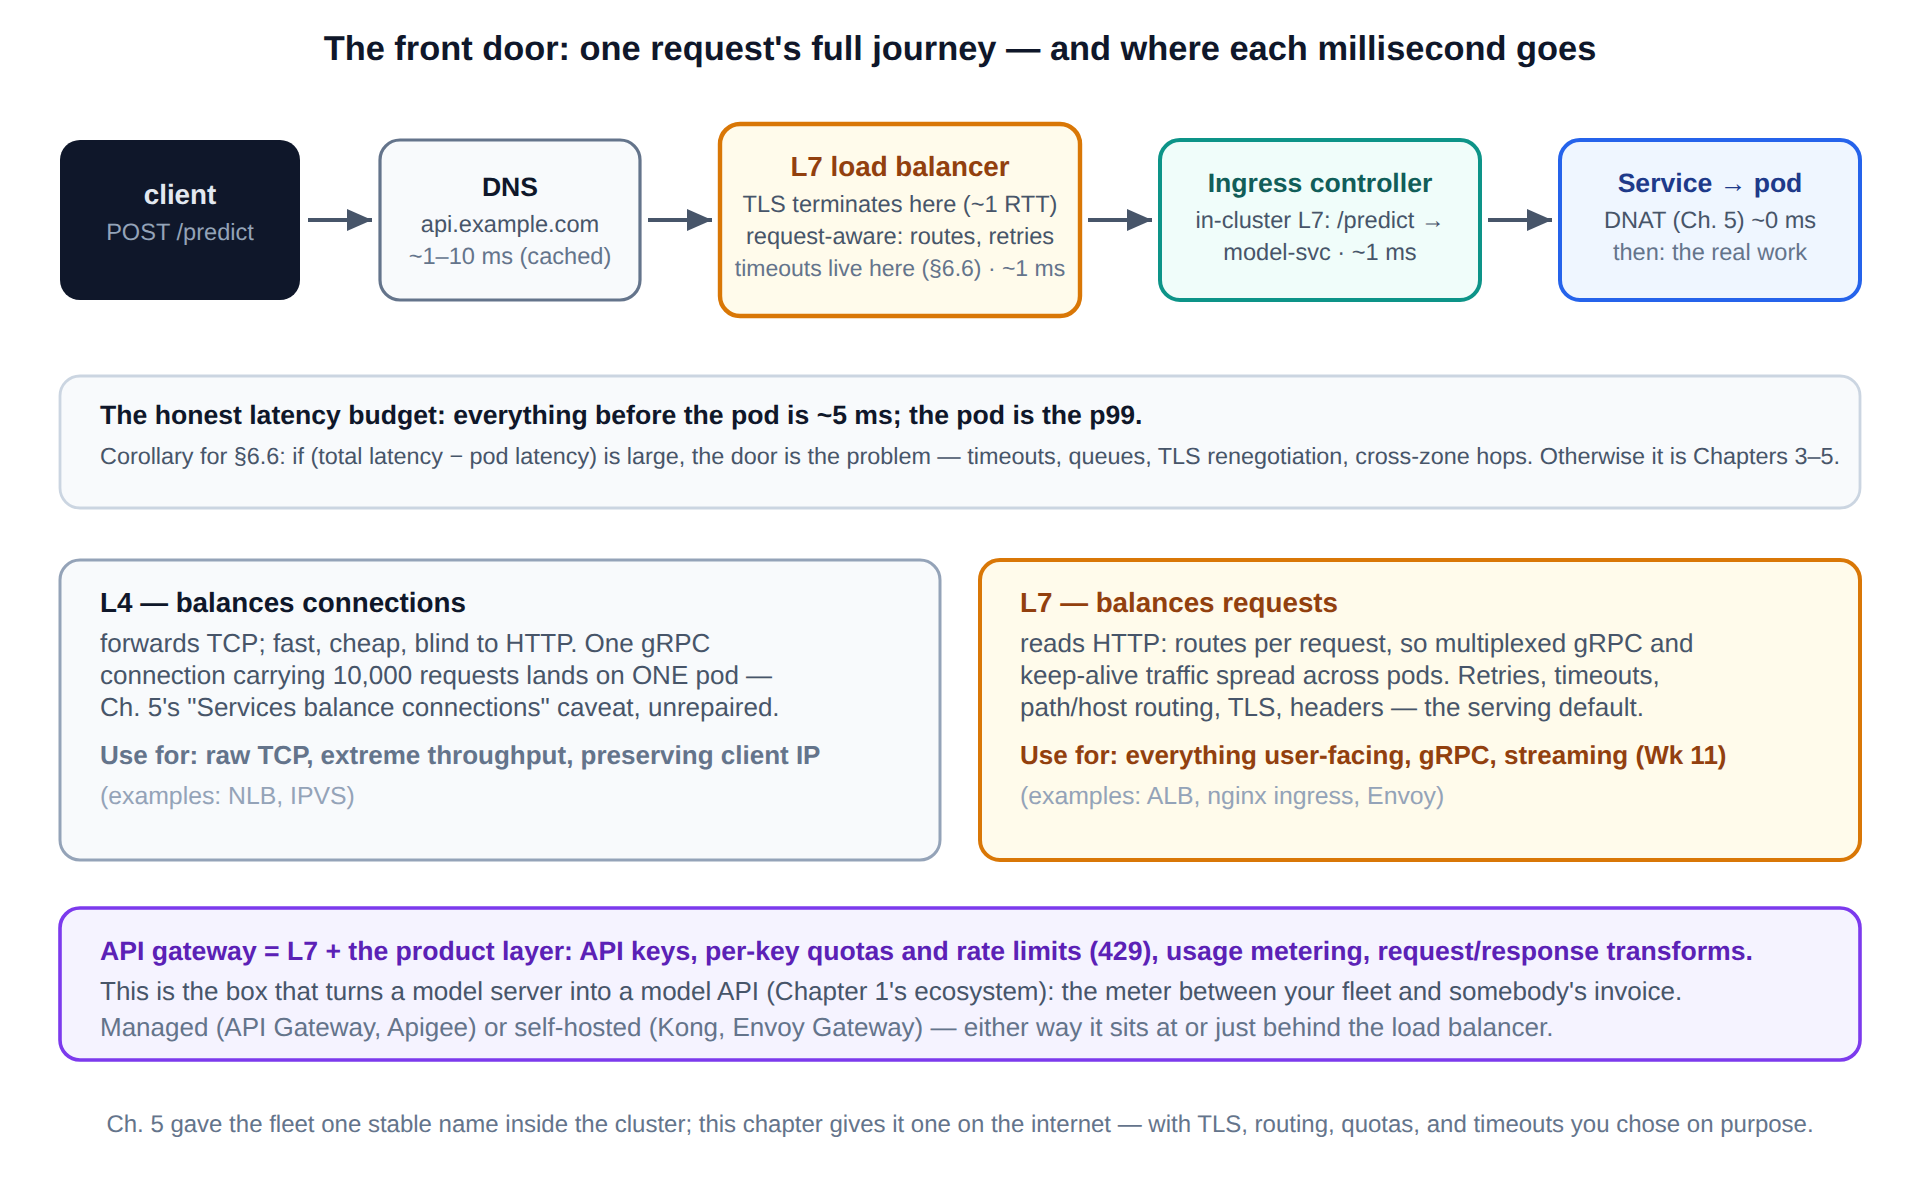
\includegraphics{figures/fig6-5_frontdoor.png}}\\[3pt]
  \figcaption{Figure 6-5  The request's journey: DNS → L7 load balancer (TLS, timeouts) → Ingress (in-cluster routing) → Service → pod. Everything before the pod costs \textasciitilde{}5 ms; the pod is the p99 — a fact §6.6 turns into a diagnostic.}
\end{tbbfigure}

\subsection*{L4 versus L7: connections versus requests}

Load balancers split into two species by \textit{what they read}. An \textbf{L4 balancer} operates on transport: it forwards TCP connections and never parses a byte of HTTP — blindingly fast, cheap, protocol-agnostic, and exactly as smart as that sounds. An \textbf{L7 balancer} terminates the connection, \textit{reads the requests}, and makes a fresh decision per request: route by path or host, retry idempotent failures, inject headers, terminate TLS, speak HTTP/2 to clients and HTTP/1.1 to pods. The distinction pays off precisely where Chapter 5 left a caveat. A Service (kube-proxy DNAT) balances \textbf{connections} — so one long-lived gRPC channel carrying ten thousand multiplexed requests lands them all on a single pod, and a fleet behind keep-alive clients can be wildly unbalanced while every dashboard says "healthy." An L7 hop re-balances at the \textbf{request} level and repairs exactly this — which is why gRPC and streaming workloads (Week 11) treat an L7 proxy not as an accessory but as a requirement. The practical pairing: L4 in front for raw packet plumbing when needed (or as the cloud entry to an in-cluster L7), L7 wherever requests are the unit that matters — which in serving is nearly everywhere.

\subsection*{Ingress: one door, many Services}

Provisioning one cloud load balancer per Service is the expensive habit beginners pick up from tutorials (each LB is a billed resource with its own IP and idle cost). Kubernetes' answer is the \textbf{Ingress}: a routing object — host and path rules mapping to Services — realized by an \textbf{ingress controller} (nginx, Envoy-based controllers, or a cloud controller that programs an ALB directly). One load balancer enters the cluster; the controller fans requests out to any number of Services; TLS certificates attach per host (and \code{cert-manager} automates their issuance and renewal — run it once in the lab and never hand-manage a certificate again):

\begin{terminalbox}
\begin{Verbatim}[breaklines=true,breakanywhere=true,fontsize=\small,formatcom=\color{tbbtermfg},codes=\tbbcodeactive]
apiVersion: networking.k8s.io/v1
kind: Ingress
metadata:
  name: serving-ingress
  annotations:
    nginx.ingress.kubernetes.io/proxy-read-timeout: "120"
spec:
  tls:
  - hosts: [ api.example.com ]
    secretName: api-tls            # cert-manager fills this
  rules:
  - host: api.example.com
    http:
      paths:
      - path: /predict
        pathType: Prefix
        backend: { service: { name: model-svc, port: { number: 80 } } }
      - path: /embed
        pathType: Prefix
        backend: { service: { name: embed-svc, port: { number: 80 } } }

$ curl -sv https://api.example.com/predict -d '{"x":[1,2]}' 2>&1 \
    | grep -E "subject:|HTTP/"
*  subject: CN=api.example.com     # real TLS, terminated at the door
< HTTP/2 200
\end{Verbatim}
\end{terminalbox}
\figcaption{Transcript 6-8  One Ingress: TLS for the host, path routing to two model Services, and a timeout annotation you set on purpose (the default would not survive §6.6's incident). One LB now fronts the whole namespace.}

\subsection*{The API gateway: where the product lives}

Above routing sits the \textbf{API gateway} — functionally an L7 proxy that also implements the \textit{product}: API keys and authentication, per-key rate limits and quotas (the \code{429 Too Many Requests} your clients will learn to respect), usage metering (per key, per route, per token — the raw material of an invoice), request validation and transformation. Managed offerings (AWS API Gateway, Apigee) and self-hosted ones (Kong, Envoy Gateway) differ in operations, not concept. For this course the gateway closes a loop opened in Chapter 1: the "model API ecosystem" you buy from — metered tokens, tiered quotas, keys — is \textit{this box}, in front of someone else's fleet. The course project requires a minimal version of the same: your model, behind TLS, with a key and a quota, is the difference between "a container that answers curl" and "a service someone could be billed for." A note on redundancy: gateway, ingress, and mesh (Week 14) all speak L7, and mature stacks deliberately collapse layers — the rule of thumb is \textit{one owner per concern} (TLS terminates once; rate limits live in one place; retries live in one place), not one box per acronym.

\subsection*{Timeouts, retries, and draining: the settings that break inference}

Front doors ship with defaults tuned for web pages — tens of kilobytes, hundreds of milliseconds — and model serving violates every assumption in that sentence. Three settings do most of the breaking. \textbf{Request timeout}: an LB will abandon an upstream that has not answered within (commonly) 30–60 s, returning \code{504}. Chapter 3 taught you inference latency has a \textit{shape} — batch- and length-scaled spikes — so the timeout must clear your honest p99 at worst-case input (Chapter 1's SLO discipline), or long requests die at the door while the GPU finishes work nobody will receive. \textbf{Idle timeout}: separately, most LBs reap connections that move \textit{no bytes} for N seconds (ALB default: 60). A streaming LLM response (Week 11) that pauses 70 s mid-generation between tokens trips it — the connection is cut at \textit{exactly} N seconds, the tell §6.6 teaches — fixed by raising the idle timeout or emitting keep-alive frames. \textbf{Retries}: an L7 door can retry failures invisibly, which is a gift for idempotent GETs and a hazard for inference — a retried 30-second generation \textit{doubles} GPU load precisely when the system is slow, and retry-on-timeout at two layers (gateway × client) multiplies: 3 × 3 = nine attempts per user action. The discipline is a \textbf{retry budget}: retry only connection-level failures (never timeouts) at one layer only, with jittered backoff — Week 9's load tests will show you a retry storm on purpose so you recognize the waveform.

The fourth setting earns its own paragraph because it explains a symptom every team eventually meets: \textbf{502 spikes exactly during rollouts.} Two draining clocks must agree. The LB de-registers a terminating pod after its own delay (\code{deregistration delay} / connection draining); Kubernetes kills the pod after \code{terminationGracePeriodSeconds} (Chapter 5's tape). If the pod dies while the LB still considers it a valid target — grace too short, delay too long, or a server that exits the instant it sees SIGTERM instead of draining (Chapter 3's handler, again) — in-flight requests hit a corpse and the door reports 502. The fix is alignment: readiness fails first (endpoints removal — traffic stops arriving), then drain in-flight work, then exit, with the grace period longer than the longest honest request. Every layer of this sentence is a chapter you have already read; the front door merely makes misalignment visible to customers.

\begin{terminalbox}
\begin{Verbatim}[breaklines=true,breakanywhere=true,fontsize=\small,formatcom=\color{tbbtermfg},codes=\tbbcodeactive]
# the streaming incident, reproduced on purpose (lab, part C):
$ time curl -sN https://api.example.com/generate -d '{"n_tokens": 999}'
...tokens......tokens.......                       # then silence...
curl: (18) transfer closed with outstanding read data remaining
real  1m0.02s                       # <- suspiciously exactly 60s
# repeat it: 60.01s. 60.02s. the roundness IS the diagnosis:
# no bytes moved for idle-timeout seconds -> the LB reaped it.
$ kubectl annotate ingress serving-ingress \
    nginx.ingress.kubernetes.io/proxy-read-timeout="300" --overwrite
$ time curl -sN https://api.example.com/generate -d '{"n_tokens": 999}'
real  1m34.8s                       # the stream now outlives its pauses
\end{Verbatim}
\end{terminalbox}
\figcaption{Transcript 6-9  The idle-timeout cut: a stream that dies at exactly 60.0 s, twice, is not a bug in your server — it is a default at the door. Week 11's token streams live or die on this setting.}

\begin{calloutbox}{tbbpurple}{tbbpurplefill}
{\normalsize\bfseries\color{tbbpurple}Think About It}\par\vspace{3pt}
\begin{tbbitemize}
  \item Health checks are requests too: 2 LB nodes × every 10 s × 20 targets, plus readiness probes from kubelets. Compute the background QPS, then name the mistake that turns health checks into real load (hint: an expensive /healthz that runs a forward pass).
  \item Design the timeout ladder for a service whose p99 is 8 s but whose worst legal request (max batch, max length) is 45 s: client timeout, gateway timeout, LB request timeout, uvicorn timeout. Which must be largest, and why is the ordering not optional?
  \item Your gateway retries connection failures once; a client library retries twice on any 5xx; the mesh (Wk 14) will add its own. A node dies under peak load. Sketch the request multiplication and the load the fleet actually sees — then write the one-sentence retry policy you would enforce.
\end{tbbitemize}
\end{calloutbox}

\section{The Perimeter: VPC, Security Groups, and the Cheap Path}

Everything so far assumed packets may flow; this section decides \textit{which} packets. The unit of decision is the \textbf{VPC} — your private slice of the cloud's network: an address space you choose (say \code{10.0.0.0/\allowbreak 16}), carved into \textbf{subnets} (per availability zone), stitched together by \textbf{route tables}. Two route-table entries define the two subnet species: a \textbf{public subnet} routes \code{0.0.0.0/\allowbreak 0} to an \textit{internet gateway} (things in it can have public IPs and be reached from outside); a \textbf{private subnet} has no such route — its instances have no public IPs and are unreachable from the internet \textit{by construction}, not by firewall diligence. The serving posture falls out immediately, and Figure 6-6 draws it: \textbf{the load balancer is the only public thing; the GPU fleet lives private.} A \$30/hour node with a public IP is an attack surface with a billing account; a private one is not reachable to attack.

\begin{tbbfigure}
  \adjustbox{max width=0.94\linewidth,max totalheight=0.46\textheight}{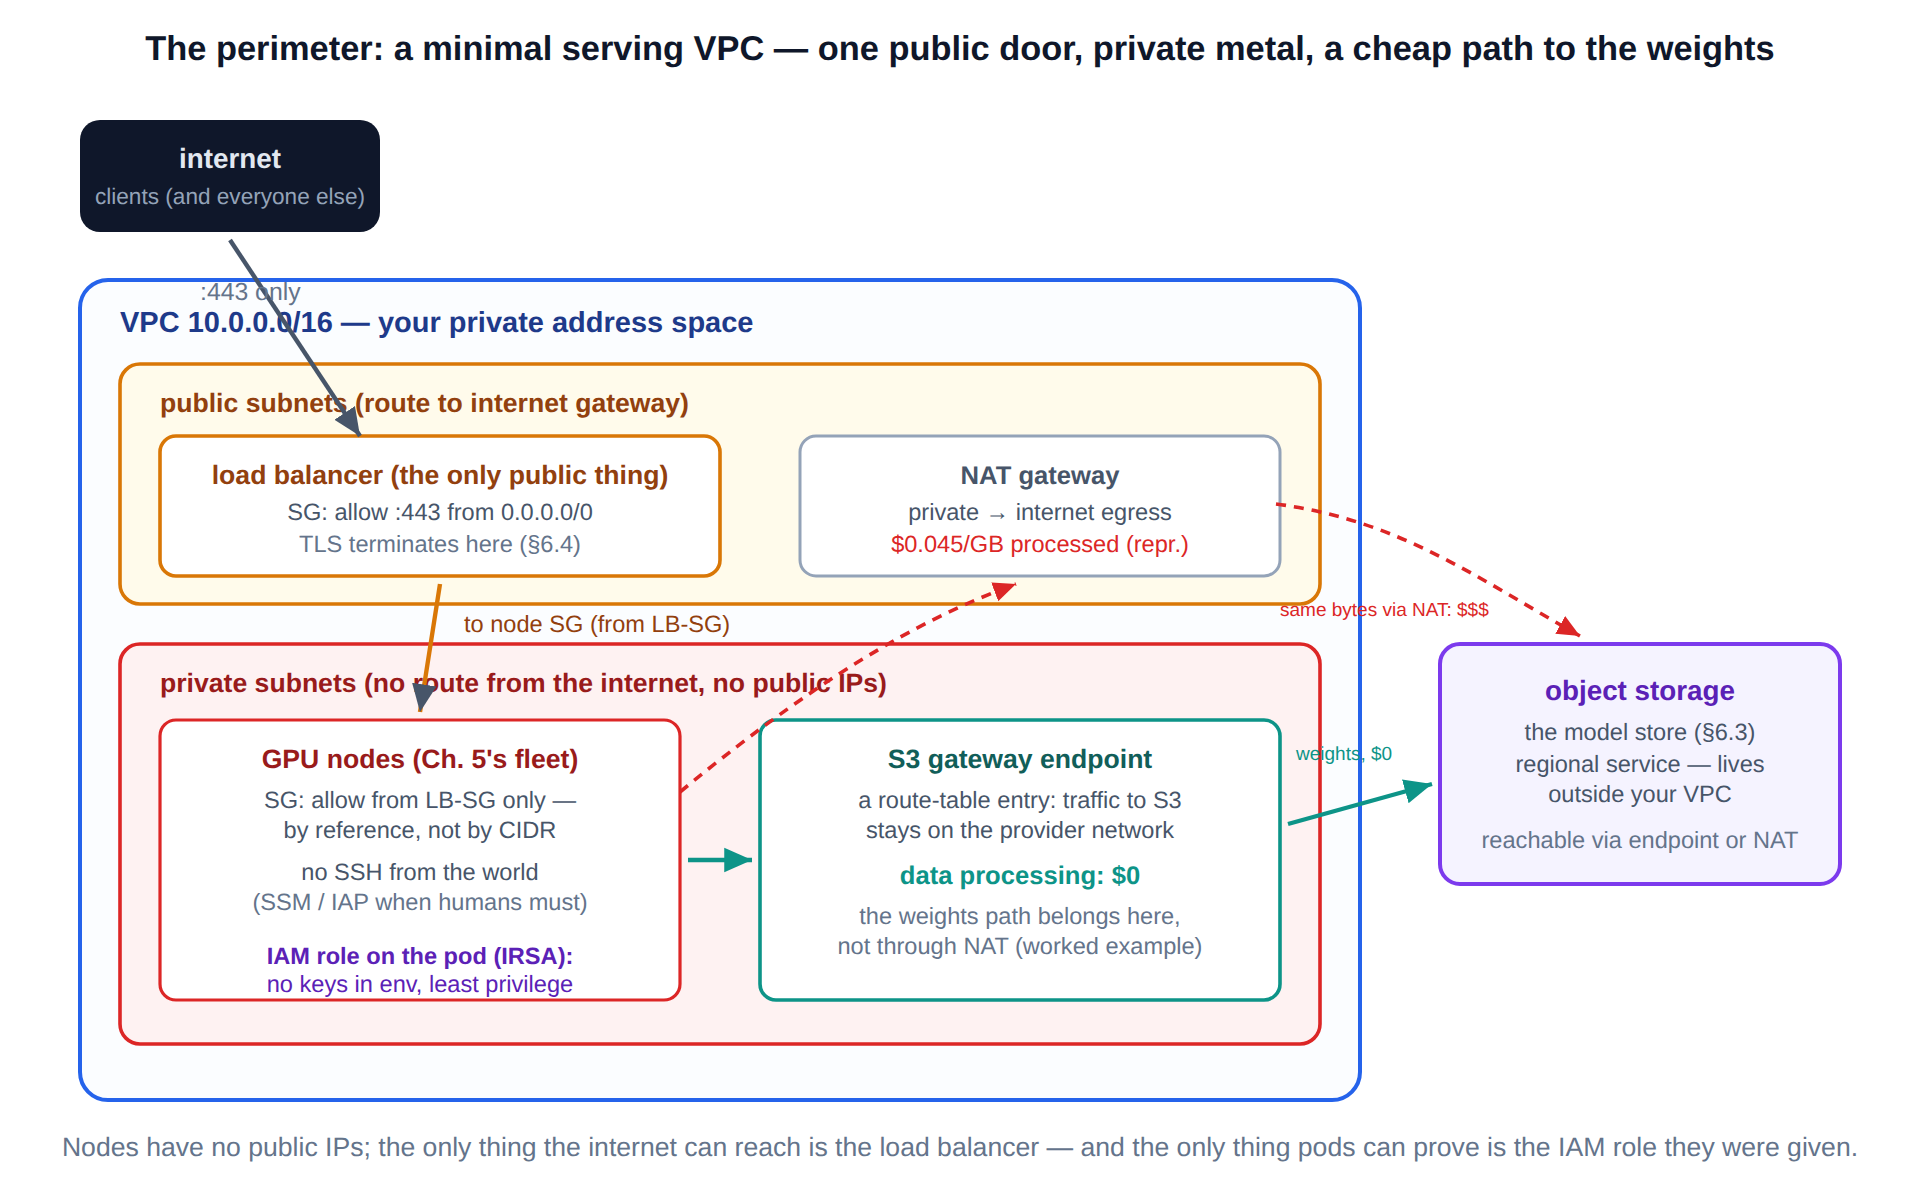
\includegraphics{figures/fig6-6_vpc.png}}\\[3pt]
  \figcaption{Figure 6-6  The minimal serving VPC: one public door (the LB), private metal (the fleet), and two ways to reach the model store — the free gateway endpoint and the metered NAT detour. Choose deliberately.}
\end{tbbfigure}

\subsection*{Security groups: stateful allow-lists, chained by reference}

Within the VPC, \textbf{security groups} (SGs) are the per-instance firewall — three properties carry everything. They are \textbf{allow-only}: an SG lists what may connect (port, protocol, source); everything unlisted is denied, so there are no "deny rule ordering" puzzles. They are \textbf{stateful}: if an inbound connection is allowed, its reply packets flow automatically — the cloud tracks connections exactly like Chapter 3's conntrack in the \code{-p 8080:8000} walkthrough, one abstraction up. And — the property that makes architectures readable — \textbf{sources can be other SGs, not just CIDR ranges.} The serving chain is three sentences: the LB's SG allows \code{:443} from \code{0.0.0.0/\allowbreak 0}; the nodes' SG allows the service port \textit{from the LB's SG} (by reference — not from an IP range that silently changes when the LB scales or moves); nothing allows SSH from anywhere (humans enter via SSM/IAP session tooling, audited, when they must). Reference-chaining means the intent survives infrastructure churn: "nodes accept traffic \textit{from the load balancer}" stays true no matter what IPs the balancer holds tomorrow. (Network ACLs — stateless, subnet-level, rule-numbered — exist beneath SGs; convention: leave them open, express intent in SGs, reach for NACLs only for blunt subnet-wide bans.)

\begin{terminalbox}
\begin{Verbatim}[breaklines=true,breakanywhere=true,fontsize=\small,formatcom=\color{tbbtermfg},codes=\tbbcodeactive]
# perimeter, demonstrated: (1) the node, from the internet:
$ curl -m 5 http://203.0.113.40:30080/predict
curl: (28) Connection timed out       # no route, no public IP. good.
# (2) the door, from the internet:
$ curl -s https://api.example.com/predict -d '{"x":[1,2]}'
{"y": 0.87, "model": "v8"}            # the one sanctioned path
# (3) identity, from inside a pod - no keys anywhere:
$ kubectl exec -it model-server-...-2xk4p -- \
    aws sts get-caller-identity --query Arn --output text
arn:aws:sts::1234:assumed-role/model-server-irsa/...
$ kubectl exec -it model-server-...-2xk4p -- \
    aws s3 ls s3://ml-models/bert-classifier/v8/   # allowed prefix
2026-07-02  461301120 model.safetensors
$ kubectl exec -it model-server-...-2xk4p -- \
    aws s3 ls s3://corp-finance-exports/
An error occurred (AccessDenied)      # least privilege, working
\end{Verbatim}
\end{terminalbox}
\figcaption{Transcript 6-10  The perimeter in three probes: nodes unreachable from outside, the LB answering, and a pod whose only credential is a scoped IAM role it cannot exfiltrate — because it was never a secret to begin with.}

\subsection*{Identity without keys — and the path the weights should take}

The transcript's third probe deserves unpacking, because credential handling is where serving systems most often embarrass their teams. The anti-pattern is an access key in an environment variable: long-lived, copy-pasteable, leaked by every \code{kubectl describe} and crash dump, rotated never. The pattern is \textbf{workload identity} (IRSA on EKS, Workload Identity on GKE): the pod's \textit{service account} — a Kubernetes identity from Chapter 5's object zoo — is bound to an IAM role, and the cloud SDK inside the pod obtains short-lived credentials automatically through the token chain. Nothing to leak, nothing to rotate, and — the operationally precious part — \textbf{least privilege becomes per-workload}: the model-server role can read \code{ml-models/\allowbreak bert-classifier/\allowbreak *} and nothing else, the loader can read but never write, the training pipeline (elsewhere) can write new prefixes but never overwrite — turning §6.3's immutability discipline from a team norm into an enforced property.

Finally, the money paragraph. Traffic from private subnets to the internet exits through a \textbf{NAT gateway}, and NAT gateways bill \textbf{per gigabyte processed} (\textasciitilde{}\$0.045/GB, representative) on top of hourly cost. Here is the trap: S3 is \textit{outside} your VPC, so a private node's S3 traffic — your 13 GB weight pulls — takes the NAT path \textit{by default}. The fix is a \textbf{gateway VPC endpoint}: a route-table entry that sends S3/DynamoDB-bound traffic across the provider's backbone directly, with \textbf{zero data-processing charge} and typically better throughput. It is arguably the highest-ROI single line of network configuration in ML infrastructure:

\begin{calloutbox}{tbbred}{tbbamberfill}
{\normalsize\bfseries\color{tbbamberdark}Worked example — the NAT tax on weights}\par\vspace{3pt}
A 20-node fleet re-pulls a 13 GB model at each daily deploy, plus autoscaling churn — call it 25 node-pulls/day: \textbf{325 GB/day} of S3 → node traffic.

\begin{tbbitemize}
  \item \textbf{Via NAT gateway:} 325 GB × \$0.045 ≈ \$14.6/day ≈ \textbf{\$440/month} — for bytes that never left the provider's network. (Plus the NAT's \textasciitilde{}\$0.045/hour ≈ \$32/month base.)
  \item \textbf{Via S3 gateway endpoint:} the same bytes, \textbf{\$0.00} — one route-table entry at creation time.
\end{tbbitemize}

Same architecture, same traffic, \textasciitilde{}\$5,000/year difference — and the failure is silent: everything \textit{works} through NAT, it just bills. Audit rule: private subnets that talk to S3 get a gateway endpoint on day one. (Cross-region is a separate tax: keep the model store in the fleet's region, or pay \textasciitilde{}\$0.02/GB and add latency — a Week 12 multi-region topic.)
\end{calloutbox}

\vspace{3.0pt}

\begin{calloutbox}{tbbpurple}{tbbpurplefill}
{\normalsize\bfseries\color{tbbpurple}Think About It}\par\vspace{3pt}
\begin{tbbitemize}
  \item Why is "node-SG allows traffic from LB-SG" strictly better than "from the LB subnets' CIDR"? Give the failure that CIDR rules develop over time, and the reason SG references cannot develop it.
  \item An attacker achieves code execution inside a serving pod (a malicious pickle — Week 7's format warning made real). Compare the blast radius under (a) an access key in env with s3:* permissions, and (b) IRSA scoped to read-only on one prefix. What can they reach in each case — and what does Chapter 3's shared-kernel caveat add?
  \item Your bill shows the NAT gateway as the third-largest line item, behind GPUs and ahead of storage. Reconstruct the likely traffic (weights? image pulls? pip installs at build time? telemetry?) and name which of those the gateway endpoint fixes versus which need a registry mirror or an interface endpoint instead.
\end{tbbitemize}
\end{calloutbox}

\section{Reading the Front Door: A Status-Code Field Guide}

Chapter 5's field guide taught you to read pod states from inside the cluster. This chapter's failures announce themselves from the \textit{outside} — a user, a synthetic check, or Week 14's alerting hands you a status code and nothing else. The good news mirrors Chapter 5's: \textbf{the code localizes the failure} before you have run a single command, because each layer of §6.4's door can only fail in its own vocabulary. And one move splits the search space in half before any forensics: \textbf{repeat the request from inside} (\code{kubectl port-forward} straight to a pod). Inside-OK + outside-broken means the door — TLS, routing, timeouts, health checks, perimeter. Both-broken means the fleet, and you are back in Chapter 5's guide with a head start (Figure 6-7).

\begin{tbbfigure}
  \adjustbox{max width=0.94\linewidth,max totalheight=0.46\textheight}{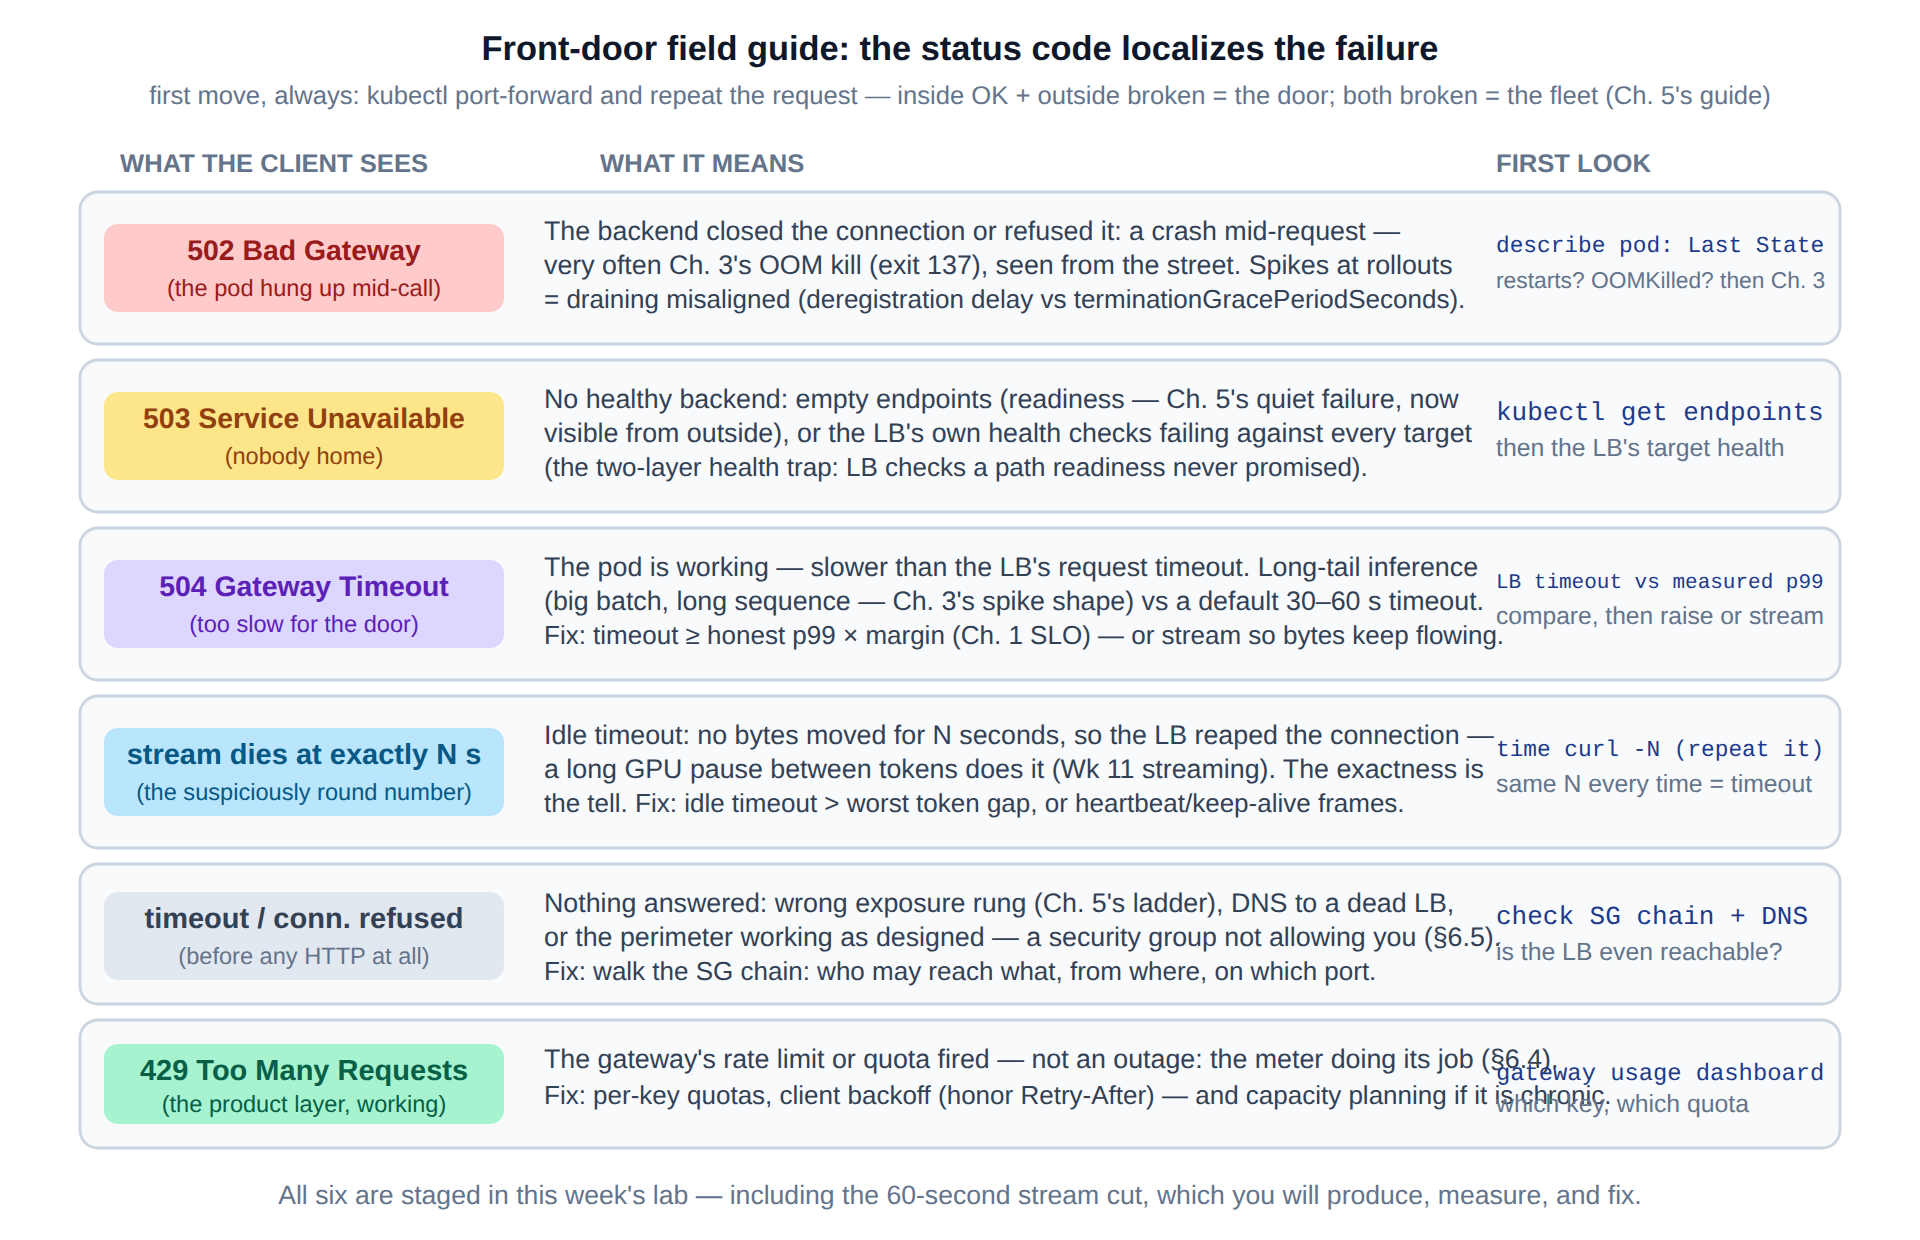
\includegraphics{figures/fig6-7_fieldguide.png}}\\[3pt]
  \figcaption{Figure 6-7  The decode table: 502 (the pod hung up), 503 (nobody home), 504 (too slow for the door), the stream cut at exactly N seconds, the silent connection timeout, and 429 (the meter, working). All staged in the lab.}
\end{tbbfigure}

\subsection*{The forensic walkthrough: a 503 with green dashboards}

\begin{terminalbox}
\begin{Verbatim}[breaklines=true,breakanywhere=true,fontsize=\small,formatcom=\color{tbbtermfg},codes=\tbbcodeactive]
$ curl -s -o /dev/null -w "%{http_code}\n" \
    https://api.example.com/predict -d '{"x":[1,2]}'
503                                  # "Service Unavailable" - from whom?
$ kubectl get pods -l app=model      # the fleet looks... fine?
NAME                            READY   STATUS    RESTARTS   AGE
model-server-59d8c7f9b6-2xk4p   1/1     Running   0          3h
model-server-59d8c7f9b6-m7qvw   1/1     Running   0          3h
$ kubectl port-forward pod/model-server-59d8c7f9b6-2xk4p 8000:8000 &
$ curl -s -o /dev/null -w "%{http_code}\n" \
    localhost:8000/predict -d '{"x":[1,2]}'
200                                  # inside OK + outside broken = DOOR
$ kubectl describe ingress serving-ingress | grep -A2 Backends
  /predict   model-svc:80   (<none>)          # <- the controller sees
$ kubectl get endpoints model-svc               #    no endpoints...
NAME        ENDPOINTS   AGE
model-svc   <none>      3h                      # Ch. 5's quiet failure -
# a readiness typo after this morning's change - now visible as a 503
# to every customer. fix the probe path; endpoints repopulate; 200.
\end{Verbatim}
\end{terminalbox}
\figcaption{Transcript 6-11  The split move in action: 503 outside, 200 via port-forward → the door. Then the door's own evidence chain: the ingress backend list and the empty endpoints — Chapter 5's quiet failure, seen from the street.}

Walk the chain the way the transcript does and each hop answers one question. The \textbf{status code} names the failing layer's vocabulary: \code{503} is a proxy saying "I have no healthy upstream" — which points at endpoints, readiness, or the LB's own health checks, never at DNS or TLS. The \textbf{port-forward probe} proves the pods can serve, converting "the API is down" into "the door has nobody to send to." And the \textbf{endpoints check} — Chapter 5's single highest-value habit — finds the cause. Two chapters, one diagnostic language: this is what it means for the infrastructure half of the course to be \textit{complete}.

\subsection*{The rest of the codebook, with their Chapter 3–5 roots}

\begin{tbbitemize}
  \item \textbf{502 Bad Gateway — the pod hung up mid-call.} The door had a connection; the backend closed it or refused it. Roots you already know: a crash mid-request — very often Chapter 3's OOM kill (exit 137: check \code{Last State} first) — or the rollout misalignment of §6.4 (pod killed while the LB still targets it: compare deregistration delay to \code{terminationGracePeriodSeconds}, and confirm the server drains on SIGTERM). \textit{502s that spike at deploy time are a draining bug until proven otherwise.}
  \item \textbf{504 Gateway Timeout — too slow for the door.} The pod is working; the door gave up first. Chapter 3 gave inference latency its spike shape (batch × sequence); Chapter 1 gave you the SLO language. The fix conversation is "raise the LB/ingress request timeout above honest worst-case p99, or bound the inputs, or stream so bytes keep flowing" — never "add a retry," which doubles GPU load exactly when the system is slowest (§6.4's budget).
  \item \textbf{The stream that dies at exactly N seconds} — §6.4's idle timeout, and the roundness is the entire diagnosis. Reproduce twice, read the number, raise the idle timeout or add keep-alive frames. Week 11's token streams make this the most-reproduced transcript in the course.
  \item \textbf{Connection timeout / refused — before any HTTP.} Nothing answered: wrong exposure rung (Chapter 5's ladder), DNS pointing at a deleted LB, or §6.5's perimeter \textit{working as designed} against you (an SG that never allowed your office range, a private endpoint you assumed was public). Walk the SG chain: who may reach what, from where, on which port.
  \item \textbf{429 Too Many Requests — the product layer, functioning.} The gateway's per-key quota fired. Not an outage: the meter protecting the fleet (and the invoice). Client fix: honor \code{Retry-After}, add jittered backoff. Operator fix: per-key quotas that match reality, and capacity planning if 429s are chronic at normal usage.
\end{tbbitemize}

\subsection*{The two-layer health trap}

One failure deserves its own subsection because it is invisible from inside. The cloud LB runs \textbf{its own health checks} against targets, independent of Kubernetes readiness. Two sources of health truth drift: the LB checks \code{/\allowbreak health} (a path your server never implemented — 404 is "unhealthy"), or checks the node's NodePort on a node whose kube-proxy routes elsewhere, or uses a stricter timeout than readiness. Result: \textbf{kubectl shows everything Ready; the LB shows zero healthy targets; customers see 503} — Transcript 6-11's symptom with a different root, and \code{kubectl get endpoints} comes back \textit{populated}, which is precisely what makes it disorienting. The rule that prevents it: \textbf{one health endpoint is the single source of truth} — the LB's check path, the readiness probe, and the gateway's check all point at the same \code{/\allowbreak ready}, with the same meaning. When the lab stages this, note where the evidence lives: not in Kubernetes at all, but in the LB's target-health console — the first time this course has sent you to a control panel outside the cluster, and a preview of Week 14's theme that observability must cover every layer that can say no.

\begin{tbbtablewrap}
  \begin{tabular}{@{}>{\raggedright\arraybackslash}m{\dimexpr 0.2181\tbltextwidth-2\tabcolsep\relax} >{\raggedright\arraybackslash}m{\dimexpr 0.3670\tbltextwidth-2\tabcolsep\relax} >{\raggedright\arraybackslash}m{\dimexpr 0.4149\tbltextwidth-2\tabcolsep\relax}@{}}
  \arrayrulecolor{tbbnavy}\specialrule{1pt}{0pt}{0pt}
  \rowcolor{tbbtablehead}{\centering \bfseries\color{tbbnavy}Signal} & {\centering \bfseries\color{tbbnavy}The door is saying} & {\centering \bfseries\color{tbbnavy}First look} \\
  \arrayrulecolor{tbbnavy}\specialrule{0.7pt}{0pt}{2pt}
  {\textbf{502}} & {backend closed/refused mid-call} & {pod restarts, Last State (OOM 137?); rollout draining alignment} \\
  \arrayrulecolor{tbbtableborder}\hline
  {\textbf{503}} & {no healthy upstream at all} & {kubectl get endpoints; then the LB's target health (two-layer trap)} \\
  \arrayrulecolor{tbbtableborder}\hline
  {\textbf{504}} & {upstream slower than my timeout} & {LB/ingress timeout vs measured worst-case p99} \\
  \arrayrulecolor{tbbtableborder}\hline
  {\textbf{cut at exactly N s}} & {no bytes for N s → idle reap} & {time curl -N, twice; raise idle timeout / keep-alives} \\
  \arrayrulecolor{tbbtableborder}\hline
  {\textbf{timeout, no HTTP}} & {you never reached me} & {DNS → SG chain → exposure rung (Ch. 5 ladder)} \\
  \arrayrulecolor{tbbtableborder}\hline
  {\textbf{429}} & {quota enforced (by design)} & {gateway usage per key; client backoff w/ Retry-After} \\
  \arrayrulecolor{tbbnavy}\specialrule{1pt}{2pt}{0pt}
  \end{tabular}\par
  \figcaption{Table 6-3  The door's error vocabulary, compressed}
\end{tbbtablewrap}

\begin{calloutbox}{tbbpurple}{tbbpurplefill}
{\normalsize\bfseries\color{tbbpurple}Think About It}\par\vspace{3pt}
\begin{tbbitemize}
  \item A user reports intermittent 502s, \textasciitilde{}1\% of requests, uncorrelated with deploys. Pod restarts are zero. Build the suspect list from this section (hint: think about \textit{which} pods serve long requests, LB connection reuse, and uvicorn worker recycling) and the measurement that discriminates.
  \item Synthetic checks (Wk 14) should catch each row of Table 6-3 \textit{before customers do}. Design three probes — path, frequency, alert condition — that together cover 503, 504, and the stream cut, and state which layer each probe must run outside of to be valid.
  \item The two-layer health trap put the evidence outside Kubernetes. List every layer in Figure 6-5 that keeps state a kubectl user cannot see, and what "green here, red there" means for each.
\end{tbbitemize}
\end{calloutbox}

\section{Lab: The S3-Loading Serving Structure, Completed}

The syllabus phrase for this week is "complete the serving structure that loads models from S3," and \textit{complete} is the operative word: after this lab, the course's serving skeleton — store → loader → fleet → Service → door — exists end to end on your laptop, with real measurements in every joint. The storage half runs against \textbf{MinIO}, an S3-compatible store deployed inside your minikube cluster (same API, same SDKs, \code{mc} instead of \code{aws}, zero bill); the cloud-perimeter half is a checklist against §6.5 plus an optional managed-cluster appendix for teams with credits. Work in the \code{ml} namespace throughout.

\subsection*{Part A — stand up the store; make the loader honest}

Deploy MinIO from the course manifest (a Deployment, a Service, a PVC — read it: every object is a Chapter 5 noun). Create the bucket and upload the course model \textbf{twice} — as \code{v7/\allowbreak } and \code{v8/\allowbreak } prefixes with manifests — practicing the immutability discipline from the first minute (\code{mc mb}, \code{mc cp}, \code{mc ls}). Then the measurement that anchors the week: run the provided naive loader (one stream) against the 4 GB lab model, record the time; extend it to N concurrent ranged GETs (the handout scaffolds the thread pool; you write the range arithmetic and the reassembly); sweep N ∈ \{1, 4, 8, 16, 32\}, plot seconds-vs-N, and identify the knee — then verify every file against \code{manifest.json} checksums before declaring victory. Deliverable artifact: the sweep table, plus one sentence naming your bottleneck (in-cluster MinIO usually pins the node's disk or veth before a real S3 would pin the NIC — say which, with evidence from \code{iostat}).

\subsection*{Part B — wire the pattern; deploy a model with one env change}

Wire Transcript 6-6 for real: initContainer (your Part A loader, now an image), \code{emptyDir}, \code{MODEL\_URI} env, and a \code{startupProbe} whose \code{failureThreshold × periodSeconds} you \textit{compute} from Part A's measured download+load time (show the arithmetic in a YAML comment — this is Chapter 5's stanza with this chapter's numbers in it). Deploy; verify the own-nothing audit (Transcript 6-1) on your own pod. Then the two set pieces. \textbf{Reconciliation with weight}: delete a pod mid-curl-loop and time the gap to the replacement's Ready — your first personally measured cold start; itemize it (schedule / init-download / load / warmup) into Figure 6-4's format from the pod's events and logs. \textbf{The env-only model deploy}: \code{kubectl set env MODEL\_URI=...v8/\allowbreak } under a running curl loop, capture the IMAGE column unchanged (Transcript 6-7), zero failed requests, and a served response that proves v8 answered. Then break immutability \textit{on purpose} in a scratch prefix — re-upload a changed file under the same URI, restart half the fleet, and document the two-truths symptom before deleting the scratch prefix and writing the one-line policy you violated.

\subsection*{Part C — the door, and its failure modes}

Enable the ingress addon (\code{minikube addons enable ingress}), install cert-manager with a self-signed issuer, and put Transcript 6-8's Ingress in front of \code{model-svc} — TLS included; \code{curl -v} must show your certificate. Then stage three field-guide rows and fix each: \textbf{(1) the 503 with green dashboards} — readiness path typo, diagnosed from the outside in, exactly Transcript 6-11's chain; \textbf{(2) the stream cut} — run the course image's \code{SLOW\_STREAM=90} mode behind the default 60 s proxy timeout, reproduce the cut at exactly 60 s twice, then fix with the timeout annotation and show the stream completing; \textbf{(3) the 504} — send the worst-legal request (max batch) through a deliberately short 10 s timeout, read the 504, then set the timeout from your measured worst case with margin. The perimeter closes the lab as a \textbf{checklist, not a build}: for the minikube world, write the §6.5 design you \textit{would} deploy (public/private split, SG chain by reference, gateway endpoint, IRSA role scoped to your bucket prefix) as a one-page annotated diagram; teams with cloud credits reproduce Transcript 6-10's three probes on a managed cluster in the optional appendix.

\begin{calloutbox}{tbbpurple}{tbbpurplefill}
{\normalsize\bfseries\color{tbbpurple}Lab checklist}\par\vspace{3pt}
\begin{tbbitemize}
  \item Part A artifacts: bucket listing showing v7/ and v8/ with manifests · loader concurrency sweep table + knee · checksum verification output · one-sentence bottleneck claim with iostat evidence.
  \item Part B artifacts: computed startupProbe arithmetic (in-YAML comment) · own-nothing audit of your pod · itemized cold-start bar with your numbers · env-only model deploy capture (IMAGE unchanged, zero failed requests) · the immutability-violation writeup.
  \item Part C artifacts: curl -v TLS handshake · the 503 forensic chain (outside → port-forward → endpoints) · the 60.0 s stream cut, twice, then fixed · the 504 before/after with your chosen timeout and its justification · the perimeter one-pager.
  \item Report: one page + the artifacts; each observation names its section (e.g., "the cut was at exactly 60 s — §6.4's idle timeout, §6.6's roundness tell").
  \item Cleanup: kubectl delete namespace ml; minikube addons disable ingress; minikube stop. (MinIO kept the whole week free — the habit stays anyway.)
\end{tbbitemize}
\end{calloutbox}

\vspace{3.0pt}

\begin{calloutbox}{tbbpurple}{tbbpurplefill}
{\normalsize\bfseries\color{tbbpurple}Think About It}\par\vspace{3pt}
\begin{tbbitemize}
  \item The env-only deploy rolled v7 → v8 with zero failed requests. Enumerate every mechanism that had to cooperate, across three chapters — then find the single cheapest misconfiguration that would have broken it (hint: a startupProbe budget that fits v7's size but not v8's).
  \item Scale the lab's pattern from 4 GB to 130 GB (Week 11 territory): which parts survive unchanged (layout, manifests, env coupling), which numbers must be recomputed (probe budgets, concurrency, disk), and which new machinery becomes mandatory (node caches, pre-warm pools)? Rank the changes by pain.
\end{tbbitemize}
\end{calloutbox}

\namedsection{Summary}{The Chapter in Ten Points}

\qitem{1}{\textbf{Your model server owns nothing.} Every byte in a pod is from the image, fetched at boot from a store, or disposable scratch — never unique. This is the license for all of Chapter 5's choreography: pods can be cattle only because nothing of value dies with one.}

\qitem{2}{\textbf{Storage is three contracts, not three products.} Block sells a disk (POSIX, sub-ms, one owner, pay-provisioned); object sells durable blobs behind HTTP (ranged GETs, unlimited readers, eleven nines, pay stored + requests + egress); file sells shared POSIX at \textasciitilde{}10× block price. Choose by access pattern, sharing, and price shape — with arithmetic.}

\qitem{3}{\textbf{Object storage's shape is "slow first byte, unbounded aggregate."} One stream crawls (\textasciitilde{}80 MB/s); sixteen ranged streams saturate a NIC (\textasciitilde{}1 GB/s). Every fast loader in the industry is this one observation, applied.}

\qitem{4}{\textbf{Weights are the most object-shaped bytes you own}: huge, immutable, versioned, written once, read by every replica, sequentially. The model store — one bucket, model/version/files, sha256 manifests — resolves Chapter 3 §3.4's caveat for good.}

\qitem{5}{\textbf{Versions are immutable: new version = new prefix, never overwrite.} Rolling updates, node caches, and rollback all silently depend on it — and IAM can enforce it (writers create, never overwrite).}

\qitem{6}{\textbf{Split the cadences and a model deploy stops being a software release.} Code in images, weights in the store, an env var as the only coupling: kubectl set env MODEL\_URI=...v8 rolls a new model through Chapter 5's full machinery — surge, readiness pacing, rollback — with the IMAGE column untouched. Week 13 automates this line.}

\qitem{7}{\textbf{Cold start is a sum, not a number}: schedule + image pull + weight download + load + warmup. Naive ≈ 260 s; engineered (cached image, 16-way loader, mmap) ≈ 56 s — same hardware. Each line has an owner; Week 12's scale-to-zero debate is this bar.}

\qitem{8}{\textbf{The front door is layered and its settings are serving-hostile by default.} L4 balances connections; L7 balances requests (repairing Chapter 5's gRPC caveat). Ingress gives one LB to many Services; the API gateway adds the product (keys, quotas, 429s, metering). Set request timeouts from honest worst-case p99, idle timeouts above streaming token gaps, retries on a budget — and align LB draining with terminationGracePeriodSeconds or buy 502s at every deploy.}

\qitem{9}{\textbf{The perimeter is structural, not diligent}: private subnets have no route from the internet — the LB is the only public thing. Security groups chain by reference (nodes accept from LB-SG); pods authenticate by workload identity, not keys; and the weights take the gateway endpoint, not the \$0.045/GB NAT detour (\textasciitilde{}\$5k/yr on one mid-size fleet).}

\qitem{10}{\textbf{The status code localizes the failure}: 502 = the pod hung up (OOM, draining misalignment); 503 = nobody home (endpoints, or the two-layer health trap); 504 = too slow for the door; a cut at exactly N seconds = idle timeout; 429 = the meter working. First move, always: port-forward and repeat — inside-OK + outside-broken = the door.}

\namedsection{Exercises}{}

\subsection*{A. Multiple choice}

\qitem{1}{Which byte, found inside a serving pod, violates the own-nothing principle?}

\begin{tbboptions}
  \item ① A JIT-compiled kernel cache in an emptyDir
  \item ② Weights downloaded by the initContainer at boot
  \item ③ A user's uploaded document, stored on the container filesystem for later retrieval
  \item ④ The Python interpreter, from the image
\end{tbboptions}

\qitem{2}{A PostgreSQL data directory belongs on block storage, not object storage, primarily because:}

\begin{tbboptions}
  \item ① Object storage is less durable
  \item ② The database needs random in-place writes at sub-millisecond latency — semantics object storage does not sell
  \item ③ Object storage cannot hold files that large
  \item ④ Block storage is cheaper per gigabyte
\end{tbboptions}

\qitem{3}{A 13 GB model downloads in 162 s with one stream and 17 s with sixteen ranged streams. The property of object storage this exploits is:}

\begin{tbboptions}
  \item ① Strong consistency after PUT
  \item ② High time-to-first-byte
  \item ③ Aggregate parallel throughput scales with concurrent ranged GETs, up to the client NIC
  \item ④ Lifecycle transitions to infrequent-access classes
\end{tbboptions}

\qitem{4}{Why must model-store versions be immutable (new version = new prefix)?}

\begin{tbboptions}
  \item ① S3 cannot overwrite objects
  \item ② Mid-rollout, old and new replicas of the "same version" would otherwise diverge; node caches keyed by URI would be silently poisoned; rollback targets could change under you
  \item ③ Overwriting is slower than creating new prefixes
  \item ④ Manifests only work on new prefixes
\end{tbboptions}

\qitem{5}{Clients report a streaming endpoint dies after exactly 60 seconds, every time. The most likely cause is:}

\begin{tbboptions}
  \item ① The pod is OOM-killed at 60 s
  \item ② The GPU times out
  \item ③ The load balancer's idle timeout reaping a connection that moved no bytes during a long token gap
  \item ④ DNS TTL expiry
\end{tbboptions}

\qitem{6}{A fleet in private subnets pulls weights from S3 daily. The single change that eliminates the NAT gateway's per-GB charge on that traffic is:}

\begin{tbboptions}
  \item ① Moving nodes to public subnets
  \item ② Compressing the weights
  \item ③ Adding an S3 gateway VPC endpoint to the private subnets' route tables
  \item ④ Switching the bucket to infrequent-access storage class
\end{tbboptions}

\subsection*{B. Short answer}

\qitem{1}{State the three legal provenances of bytes in a serving pod, and give one concrete example of each from this chapter's transcripts.}

\qitem{2}{Compute a cold-start budget: image 6 GB cold-pulled at 150 MB/s; weights 26 GB at one stream (80 MB/s) vs sixteen streams (800 MB/s); load 30 s; warmup 15 s; schedule 2 s. Give both totals and name the biggest single lever.}

\qitem{3}{L4 versus L7 in two sentences — then name the Chapter 5 caveat that only an L7 hop repairs, and the workload (Week 11) that makes it mandatory.}

\qitem{4}{Your rollouts produce a burst of 502s for \textasciitilde{}20 seconds. Name the two clocks that are misaligned, the Chapter 3 mechanism the server must implement for the fix to work, and the readiness-first ordering that makes draining clean.}

\subsection*{C. Essay}

\qitem{1}{"Bake the weights into the image" versus "load from a model store at boot." Argue both sides honestly — include the edge/air-gapped cases where baking wins, the cadence and registry-egress arguments where the store wins, and the cold-start arithmetic both must face. Decide for the course project and defend the decision against the strongest counterargument.}

\qitem{2}{Design the complete path for a new public model API: store layout and IAM write/read policies, loader and probe budgets, Ingress/gateway topology with TLS and quotas, VPC/SG/endpoint layout — annotating each hop with its failure mode from §6.6 and its cost line from this chapter's worked examples. One page of prose or an annotated diagram.}

\qitem{3}{"Object storage won machine learning." Evaluate: what about the contract (immutability, unlimited readers, parallel throughput, price) fits ML artifacts so well — and what costs does the fit impose (first-byte latency, cold starts, no in-place update) that the rest of the serving architecture must absorb? Use the caching ladder, the cold-start bill, and Week 11's larger models as evidence either way.}

\namedsection{Answers and Commentary}{}

\subsection*{A. Multiple choice}

\qitem{1}{\textbf{③} The upload exists nowhere else — the pod stopped being cattle, and every Chapter 5 mechanism (eviction, rollout, rescheduling) is now a data-loss path. ①, ②, ④ are the three legal provenances: scratch, fetched, image. (§6.1)}

\qitem{2}{\textbf{②} The contract clause, not the durability or size folklore: a B-tree rewrites pages in place at disk latency; object storage sells whole-object PUT/GET over HTTP. (Analytics on immutable Parquet is the counter-case that proves the rule.) (§6.2)}

\qitem{3}{\textbf{③} The object contract's shape: slow first byte, unbounded aggregate. Ranged GETs multiply streams until the client NIC (or disk) saturates — 10 Gbps ≈ 1.25 GB/s ceiling. (§6.2–6.3)}

\qitem{4}{\textbf{②} All three failures are real incidents: two-truths fleets mid-rollout, poisoned caches, mutated rollback targets. ① is false (S3 overwrites happily — that is why discipline plus IAM must forbid it). (§6.3)}

\qitem{5}{\textbf{③} The roundness is the tell: idle timeout reaps connections with no bytes in flight for exactly N seconds. Fix: raise idle timeout above the worst token gap, or emit keep-alive frames. (§6.4, §6.6)}

\qitem{6}{\textbf{③} The gateway endpoint is a route-table entry that carries S3 traffic on the provider backbone at \$0 data processing — the \textasciitilde{}\$5k/yr line-item fix. ④ changes storage cost, not transit. (§6.5)}

\subsection*{B. Short answer}

\qitem{1}{(a) From the image — /usr, the Python runtime (overlay mount, Transcript 6-1); (b) fetched at boot — the 13 GB of safetensors in /models via the initContainer; (c) disposable scratch — /dev/shm, tokenizer/JIT caches in emptyDir. Anything outside the three is a design bug. (§6.1)}

\qitem{2}{Image: 6 GB / 150 MB/s = 40 s. Weights: 26 GB / 80 MB/s = 325 s vs 26 GB / 800 MB/s ≈ 33 s. Naive: 2 + 40 + 325 + 30 + 15 = \textbf{412 s}; engineered: 2 + 40 + 33 + 30 + 15 = \textbf{120 s} (and \textasciitilde{}80 s with a node-cached image). Biggest lever: parallelizing the weight download (−292 s). (§6.3)}

\qitem{3}{L4 forwards TCP connections and never reads HTTP; L7 terminates connections and balances individual requests. The caveat: Services balance connections, so multiplexed gRPC pins to one pod — only request-level (L7) balancing repairs it; Week 11's streaming LLM traffic makes it mandatory. (§6.4)}

\qitem{4}{The LB's deregistration delay vs the pod's terminationGracePeriodSeconds. The server must actually drain on SIGTERM (Chapter 3's PID-1 handler; exec-form CMD). Clean order: readiness fails first (endpoints removal stops new traffic) → drain in-flight → exit within grace. (§6.4, §6.6)}

\subsection*{C. Essay (grading points)}

\qitem{1}{For baking: air-gapped/edge (no store reachable), single-artifact auditability, no boot-time dependency on the store's availability SLA. For the store: cadence split (model deploys without builds — Transcript 6-7), registry egress and node-disk multiplication, version explosion in image tags, Chapter 3's layer arguments. Both face the same cold-start sum — baking moves bytes to the image-pull line, it does not delete them. Full credit engages that symmetry and lands a position for the project (store, with the edge case named as an exception policy). (§6.1, §6.3)}

\qitem{2}{Look for: versioned prefixes + manifests, writer-creates/never-overwrites IAM, reader scoped per prefix; probe budgets computed from measured download+load; one LB → Ingress → Services with TLS via cert-manager, gateway for keys/quotas; private nodes, SG chain by reference, gateway endpoint on day one; per-hop failure annotations (503 endpoints, 504 timeout, cut-at-N idle, 502 draining) and cost lines (storage pennies, NAT tax avoided, LB hourly, egress on responses ≈ noise). Bonus: one health source of truth across LB/readiness/gateway. (§6.3–6.6)}

\qitem{3}{Strong answers connect contract to artifact: ML's artifacts are large, immutable, versioned, fan-out-read — the exact promise object storage sells at \textasciitilde{}\$0.023/GB-mo; and the imposed costs are real: tens-of-ms first byte and no in-place update push complexity into loaders (parallel ranged GETs), caches (the ladder), probe budgets, and Week 12's pre-warming — i.e., the architecture bends around the store rather than the reverse. Week 11 scaling (130 GB+) sharpens both sides: the store scales unbothered while every downstream number (budgets, caches, NICs) must be re-derived. Either verdict earns credit if it prices the bend. (§6.2–6.3, §6.7)}

\namedsection{Further Reading}{}

Entries tagged \textbf{[This week]} are required reading now; a \textbf{[Wk N]} tag marks material that pays off in that later week.

\begin{tbbitemize}
  \item \textbf{[This week] AWS S3 documentation: "Performance Guidelines" and "Optimizing Amazon S3 Performance"} — the primary source behind §6.3's loader: request parallelism per prefix, ranged GETs, multipart thresholds. Short, concrete, and the same ideas hold for GCS.
  \item \textbf{[This week] safetensors documentation (Hugging Face)} — the format's header layout, why mmap-ability falls out of the design, and the security argument against pickle that Week 7 will repeat with feeling.
  \item \textbf{[This week] Kubernetes docs: "Ingress", "Init Containers", and "Volumes" (emptyDir)} — the three concept pages this chapter's manifests are built from; read Ingress alongside your controller's annotation reference, because timeouts live in annotations.
  \item \textbf{AWS docs: "VPC endpoints for Amazon S3" and "NAT gateways" (pricing page included)} — fifteen minutes that recover \textasciitilde{}\$5k/yr on a mid-size fleet; the worked example of §6.5, from the vendor's own mouth.
  \item \textbf{Google SRE Book, ch. 19–20 ("Load Balancing at the Frontend" / "in the Datacenter")} — the canonical treatment of L4/L7, health checking, and draining at scale; §6.4 is the serving-sized version of these chapters.
  \item \textbf{Kleppmann, "Designing Data-Intensive Applications", ch. 3} — the storage-engines chapter: what block-backed engines actually do with those in-place writes, i.e., the other side of §6.2's contract table.
  \item \textbf{[Wk 7] ONNX / TorchScript / safetensors format comparisons (framework docs)} — next week's model-format discussion assumes this chapter's store is where formats live and convert.
  \item \textbf{[Wk 12] Cluster Autoscaler FAQ + cloud provider docs on image streaming/pre-pulling} — the cold-start bar's remaining knobs: pre-warmed pools, lazy image mounts, scale-to-zero economics.
  \item \textbf{[Wk 13] MLflow Model Registry (or equivalent) documentation} — the registry as a database of pointers into this chapter's store: stages, promotion, lineage. The mechanism stays Transcript 6-7.
\end{tbbitemize}

\vspace{5.0pt}

\begin{calloutbox}{tbbblue}{tbbbluefill}
{\normalsize\bfseries\color{tbbblue}Next chapter — Chapter 7: Serving Systems, Properly Begun}\par\vspace{3pt}
The infrastructure half of the course is complete: kernel, containers, images, orchestration, storage, and the front door. Part 2 climbs the stack and stays there. Chapter 7 opens with the serving problem itself: \textbf{online versus batch versus streaming inference} and where each earns its keep; the \textbf{latency–throughput trade-off} stated with queues rather than slogans; \textbf{SLOs and the percentile vocabulary} (p95/p99) that every later benchmark speaks; and \textbf{model formats} — ONNX, TorchScript, safetensors — with the conversion paths between them, now that you know exactly where formats live (§6.3's store) and what loads them (this chapter's loader). It is also proposal week for the team project: the SLO you promise in Week 7 is the number your Week 15 demo is graded against — choose it with Chapter 1's triangle open on the desk.
\end{calloutbox}
